\documentclass[12pt]{ociamthesis}  % default square logo 
%\documentclass[12pt,beltcrest]{ociamthesis} % use old belt crest logo
%\documentclass[12pt,shieldcrest]{ociamthesis} % use older shield crest logo

%load any additional packages
\usepackage{amssymb}
\usepackage{wrapfig}

\usepackage[hyphens]{url}
\usepackage{graphicx}
\usepackage{pdfpages}

% c#
\newcommand{\Csharp}{%
{\settoheight{\dimen0}{C}C\kern-.05em \resizebox{!}{\dimen0}{\raisebox{\depth}{\#}}}}

%input macros (i.e. write your own macros file called mymacros.tex 
%and uncomment the next line)
%\include{mymacros}

\title{Posture Behaviour at Home\\[1ex]     %your thesis title,
}   %note \\[1ex] is a line break in the title

\author{Ching Su}             %your name
\college{Human-Computer Interaction}  %your college

%\renewcommand{\submittedtext}{change the default text here if needed}
\degree{Master of Science}     %the degree
\degreedate{November 2015}         %the degree date

%end the preamble and start the document
\begin{document}

%this baselineskip gives sufficient line spacing for an examiner to easily
%markup the thesis with comments
\baselineskip=18pt plus1pt

%set the number of sectioning levels that get number and appear in the contents
\setcounter{secnumdepth}{3}
\setcounter{tocdepth}{3}

\maketitle                  % create a title page from the preamble info
\begin{dedication}
The research is dedicated to my dear family and friends here for giving me the opportunity to study in Scotland and fall in love with St Andrews.
\end{dedication}
        % include a dedication.tex file
\begin{acknowledgements}
I would like to present my deep appreciation to my supervisor Professor Aaron Quigley for his guidance of my dissertation in the summer. Without his directions and insightful suggestions I could not finish the development of the system introduced in the dissertation, which made me full of the sense of accomplishment and pleasure. Also I very appreciate the kind help from Dr. David Harris-Birtill, who provided valuable comments for my design of the evaluation and the writing of the dissertation.

It is an unforgettable year in my life to study here in St Andrews with amazing lecturers and classmates, and to finish the dissertation. I would always appreciate the knowledge and skills I learned and the experience I gained, with the sincere hope of coming back soon.
\end{acknowledgements}
   % include an acknowledgements.tex file
\begin{abstract}
\begin{abstract}
The aim of the research is to build an interactive system for posture improvement used in home setting. The target postures are defined from a trade-off between a combination of posture guideline and a predicted relaxing user experience. The posture would be observed by a Kinect. A feedback model that contains 33 feedback methods was developed to enable some appropriate methods can be chosen from for the implementation after evaluation. The feedback methods in the model have 7 targeting posture types, 5 output devices, and 3 intervention extents. A feedback with less intervention extent would be delivered earlier for reducing the interference to the users' current activity.A user study with 12 participants was carried to building a posture classification model, set the baseline of posture behaviour pattern in two scenarios, and investigate the perspectives related to the system design. 

The feedback system include three feedback methods, which are delivered by the projector and the mobile device.The feedback methods can visualise the general posture  behaviour of all the users in the environment, provide ongoing reinforcement, illustrate the impact of current posture individually, and enable active exploration of current posture.The evaluation of the system was done by the comparisons between the posture behaviour measured in the scenarios before and after the system was applied and an interview for investigating the 8 dimensions of usability of the system with 11 participants. The occurrence rate of every target posture was found decreased in every scenario, and the usability in 8 dimensions was rated 4.4 on average on a Likert 5-point scale. The posture classification model can be verified using the data from more people and an UI can be added to improve the flexibility of the system in the future.
\end{abstract}
\end{abstract}          % include the abstract

\begin{romanpages}          % start roman page numbering
\tableofcontents            % generate and include a table of contents
\listoffigures              % generate and include a list of figures
\end{romanpages}            % end roman page numbering

%now include the files of latex for each of the chapters etc
\chapter{Introduction}

\section{Background}

Postural researches from the past three decades focused on different parts of the human body and identified different factors that can influence health. The findings of Bergqvist et al.~\cite{vdt_on_musculo_disorder}, Gerr et al.~\cite{epid_musculo_disorder}, and Dunne et al.~\cite{wearable_spinal_posture} all suggest a correlation between musculoskeletal discomfort and engagement in activities employing visual display terminal (VDT) devices with unhealthy postures. Among the research, four postures, including rotate the head by too large angles, sit with the lower back not being supported, maintain a same postures for long time, and cross legs, are repeatedly proved to be related to potential musculoskeletal disorders. The techniques developed to improve posture, such as the \textit{Lumo Back}~\cite{wearable_spinal_posture}, however, only targeted one or few bad postures and had very few feedback methods. The aim of the research is to constructing a posture improvement system that could detect multiple bad postures and provide effective feedback.

\section{Motivation}
Sometimes I will also experience musculoskeletal discomfort such as sour waist and tight shoulders. I contributed the symptoms to my improper sitting posture. Even though I understand that some postures could be harmful to my body, I find it very hard to remind myself to avoid those postures while focusing on other tasks. Therefore, I believe it would be useful to have a system that can detect the postures and provide appropriate feedback.

\section{System}
In the current research, the target postures were selected from a trade-off between findings from a posture guidance review and assumed relaxing user experience. Microsoft Kinect is used to obtain posture data based on the justifications from the findings in literature review. A feedback model was constructed to provide feedback to the detected posture using different feedback methods. An initial user study was conducted to gather the target posture data to build a posture classification model. In addition, the occurrence rate of different postures in two scenarios was also measured to set the baseline of the posture behaviour pattern. The user study also investigated issues related to the system design through an interview.

The system implements three different feedback methods. They are delivered through a projector and a mobile device. The general posture behaviour of all users in the environment is visualized, showing the impact of each individual's current posture. Users can also interactively explore the type and duration of their current posture.

The system evaluation was conducted in the second user study. The participants' posture behaviour were measured in the same scenarios as those in the prior user study in order to investigate the effects of the system on the occurrence rate for the target postures. In addition, an interview were carried out to examine to the usability of the system.

\section{Objectives}
The objectives of the research are to reduce the occurrence rate of the target postures in every scenario with a positive user experience of the system. To achieve this, the system should:

\begin{enumerate}
  \item Detect health behaviours sensitively and accurately
  \item Provide real time feedback in interesting way that would not irritate or bore the users
  \item Provide effective feedback that would make the users take action on improving the target postures
\end{enumerate}

\chapter{Literature Review}

\section{Factors in health behaviours and musculoskeletal disorder}

\subsection{Head Rotation and Inclination}
Empirical evidence in the past three decades has repeatedly showed a strong causality between health-related behaviours and potential musculoskeletal disorders (MSDs) in VDT activities. Gerr, Marcus, and Monteilh~\cite{epid_musculo_disorder} published a literature review on relationships between postures of VDT activities and threats to health, suggesting high correlations between musculoskeletal problems and some particular postures. Firstly, a larger angle of head rotation or inclination was found to be correlated to a higher probability of discomfort reporting and actual clinical abnormality. The cross sectional study was conducted by Hunting et al.~\cite{constrained_postures_vdt} with 162 workers, VDTs and non-VDT users included. Secondly, Starr~\cite{posture_discomfort_vdt} showed a higher reporting probability of back pain associated to downward monitor perspective angle of VDTs operators. The investigation from 100 VDTs users suggested that upper limb postures were correlated to back and upper extremity symptoms. Results from the two researches are also supported by the findings of Coley et al.~\cite{arm_daily_activity}.

\subsection{Shoulder flexion and ulnar deviation}
Sauter et al.~\cite{work_posture_musculo_discomfort} found the relationship between higher frequency of right arm symptom occurrence and larger degree of shoulder flexion, as well as greater ulnar deviation and higher frequency of upper limb discomfort by examining 40 VDTs users.

\subsection{Arm Rest}
As the result of an literature review in arm support and arm rest design from 1982, Lueder et al. argued that having some place on the chair by appropriate height could decrease the risk of neck or shoulder discomfort~\cite{armrest_design_use}.

\subsection{Duration of engagement in VDTs activities and others}
Bergqvist, Wolgast, Nilsson, and Voss~\cite{vdt_on_musculo_disorder} carried out a study to test the muscle problem occurrence between VDT users and non-VDT users among 353 participants and no general difference between two experimental groups was found. However, when other variables of specific VDT work conditions were considered, such as using a VDT over 20 hours a week, the result showed a significant difference~\cite{vdt_on_musculo_disorder}. The findings indicate that using a VDT regularly may not necessarily cause a higher probability of threats to health, but some relevant factors, which includes long-term uses with limited rest break, repetitive movements, lower arm not supported do. All the factors may be avoided by simple behaviour improvement.

\subsection{Summary}
To conclude, although a casualty between VDT uses and risks for upper extremity musculoskeletal disorders did not be proved, the correlations between the two are repeatedly proven~\cite{epid_musculo_disorder}. Some of the factors caused to bride musculoskeletal discomfort are associated with the design of workstations, but most of them can be avoided by the improvement of posture behaviour, as postures themselves can be regarded as an independent risk variables, such as the degree of head rotation, for musculoskeletal disorders~\cite{mindandmuscle_correct_posture}. Therefore, the system would be developed to focus on the improvement of the variables.

\section{Target Postures}
Different research suggests different criteria for the postures that could threaten the health. A journal review of posture guidance is conducted to decide the appropriate criteria for good posture that maximise the effectiveness of our system. Hargrove~\cite{bad_posture_back_pain} claimed that the research results about the impact of “bad” postures are not consistent in all studies, and the presentation of a same posture for long time, no matter it is a ``good'' one or not, is one of the main causes of body stress and pain, as the support of body weight is concentrating in the same places when keeping a same posture. Therefore, performing subtle variations in any posture may help more than finding and maintaining a single perfect posture~\cite{bad_posture_back_pain}.

In addition to having some variations in a posture from time to time, three sitting posture suggestions are proposed on official website of NHS~\cite{nhs_sit_correctly}. The suggestions include supporting the lower back, placing the feet flat, and  letting the eyes level  align to the top of displays, which is an instruction for preventing a great head tilting angle~\cite{nhs_sit_correctly}. Besides, the proper viewing distance should also be cared for. Canadian Association of Optometrists (CAO) indicates that whether watching a display with a short viewing distance could result in a permanent harm of eyes, but would bring to eyestrain and fatigue~\cite{best_viewing_distance_tv}. The optimal distance for viewing a TV display suggested by CAO is five times of the width of the display, e.g. 15 feet for a 42 inches display. After the test for the suggestion, however, the researcher stated that the recommended distance of CAO, which is about 15 feet, could be too long; a distance of 10-12 feet is preferred~\cite{best_viewing_distance_tv}. According to the feedback from Torres, the optimal least distance for viewing a TV will be set as three times of the width of the display for current system application.

There still are many advises defining a good posture. However, some advices have no clear definition and guidance, such as a proper shoulder flexion and ulnar deviation. Some advises, on the other hand, is not as well supported by empirical research result, such as place the feet on floor~\cite{nhs_sit_correctly}. More importantly, the target postures for current system should come after a trade-off between a perfectly strict heath guidance and a predicted relaxing user experience. The target postures of the system to be improved are listed in Table~\ref{tab:posture_descriptions}.

\begin{table}
\centering
\begin{tabular}{|p{10cm}|p{5cm}|}
    \hline
    \textbf{Description} & \textbf{Posture}\\
    
    \hline
    Keep a same posture more than 20 minutes & Stationary\\
    \hline
    The bottom of back does not contact to the back of the chair/sofa & Slouch/\\
    , but the upper back does & Lower back not supported\\
    \hline
    Cross legs & Cross-legs \\
    \hline
    Eyes level not align to the top of displays & Low viewing height\\
     & High viewing height\\
    \hline
    Watch a display from less than 3 times of the screen width & Short viewing distance \\
    
    \hline
\end{tabular}
\caption{Target Postures of the System.}
\label{tab:posture_descriptions}
\end{table}

\section{Posture Measurements}
The first challenge of the system is to find a way to recognise target features sensitively and accurately in real time. Li and Buckle~\cite{work_musculo_risks_posture} reviewed 19 posture-based assessment methods; 10 of them can be conducted with computer-based techniques that meet our requirement for automation. One of the ten is VIRA, which is a real-time upper-body postural frequency and duration analysis using video record. VIRA was developed in 1995 and has been applied in many empirical researches, e.g. disorders of the cervicobrachial region among female workers in the electronics industry~\cite{vira_disorder_electronics}. However, the research focuses on the observation of individual parts of the body, but the current system would cover the  whole body. Dunne et al.~\cite{wearable_spinal_posture} also indicated several methods for posture measurement, among which self-administered questionnaires, professional observations and physical examinations would not be discussed here since they do not fulfill the requirement of automation for the system.

Electromyography and electro-goniometry could be excluded as well as their measuring sensors need to be in contact with users’ skin, which would interfere the tasks that the users are doing. A measurement device of the system that enable remote sensing is preferred as it could influence users; current activities at the least extent. In conclusion, 3D kinematics would be the best method to be applied as the input method of current system among the candidates proposed by Dunne et al.~\cite{wearable_spinal_posture}.

The observation of the system should cover not only the posture behaviours of users, but also the context of the environment. An ontology-based approach for context modelling, which is identified as the best approach in context-modelling by the researchers, was introduced~\cite{contextaware_reminder_living_behaviour}. Zhang et al.~\cite{contextaware_reminder_living_behaviour} suggests that a system should consider “where the user is”, “what the user is doing?” and “where it is necessary to deliver a reminder” to provide a feedback appropriately. The performance of the model is defined as the overall degree of distributed composition, partial validation, richness and quality of information, incompleteness and ambiguity, level of formality, and applicability to existing environments~\cite{contextaware_reminder_living_behaviour}.

Therefore, using 3D kinematics tool following an ontology-based approach would be an appropriate way to collect target data for the system. There are many 3D kinematics tools available currently, such as a stereo camera, a structure sensor and a Kinect. The Kinect is chosen for the system because of its large coverage, from one meter to 3 meter from the device with 54.0 degrees horizontal view and 39.1 degrees vertical view~\cite{evaluation_kinect_workspace}. The valid measurement volume of a Kinect sensor is illustrated in Figure~\ref{fig:kinect_coverage}. Besides, Kinect can detect up to six people in the room, which is more than the expected amount of people in the target environment. In addition, the price for Kinect is relatively low so that the system would be more affordable to a normal family. The reliability and validity of using Kinect for assessment of postural control are verified with high inter-trial reliability (ICC difference = 0.06 +- 0.05; range between 0.00–0.16) and concurrent validity (Pearson’s R-values > 0.90 for the majority of measurements)~\cite{validity_kinect_postural_control}.

A posture classification model using the data gathered by the Kinect would be built later in the research.

\begin{figure}[h]
\centering
    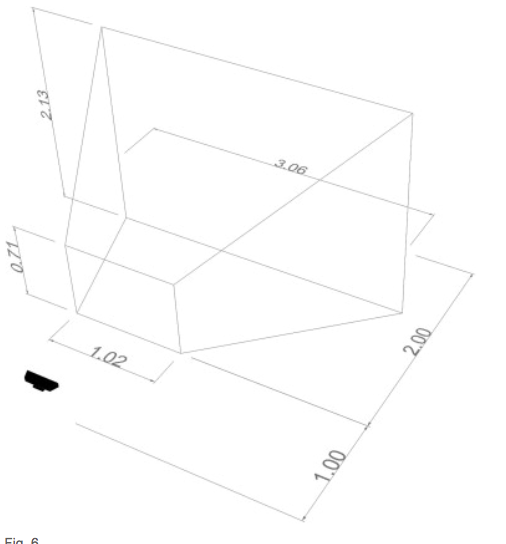
\includegraphics[width=0.5\textwidth]{figs/kinect_coverage}
\caption{The valid volume of a Kinect sensor~\cite{evaluation_kinect_workspace}}
\label{fig:kinect_coverage}
\end{figure}

\section{Posture Improvement Systems}
There have already been some techniques developed for posture improvement for the goods of human health. Lumo Back is one of the examples. It is a wearable sensor as the one developed to monitor seated spinal posture by Dunne et al.~\cite{wearable_spinal_posture}, attached on a belt to be worn on the user’s waist. It can detect slouch, and vibrate in response to the posture. In addition to the vibration feedback, it also passes the data via Bluetooth to the smartphone, and a specific application will illustrate current posture of user with the overall performance statistical pattern~\cite{review_lumo_posture_belt}. The device is light and the battery can last long. More importantly, the device is sensitive and multiple feedback can be provided~\cite{mindandmuscle_correct_posture}. However, according to Biggs~\cite{posture_saving_device}, the remainder of Lumo Back tends to lead users over-correct their postures, causing them to receive another wrong-posture feedback. Also, for users with poor postures, Lumo Back can be activated too often as well and get them annoyed.

Another technique developed for posture correction is a smartphone based real-time daily activity monitoring system. It will send a music-based alert when the system detects the user is about to fall down in order to remind them to correct their posture in time. Zhang et al.~\cite{smartphone_daily_activity_monitor} developed some algorithms for the system based on accelerometer, orientation principles and kinematical theory, for the use by different users in different environments. The judgment between a fall and a normal lying/sit-tilted is based on whether the music alarm is turned off in time~\cite{smartphone_daily_activity_monitor}. Several problems can be seen for the system. Firstly, many people may be not used to carry a smartphone by putting them in the pocket, or hold by hand all the time. Same problem will be even more apparent in the home setting. Few people tend to carry their smartphone by their bodies at home, where is the most common place for elderly, possibly the target users of the system. Secondly, the studies did not show whether feedback of the can effectively change the user's posture before they fall compared to the baseline measurement. Thirdly, the research did not run a user experience study to evaluate the usability of the system; therefore the user experience and other aspects of the system cannot be understood.

Another relevant technique to construct healthy postures is a monitor support apparatus. The monitor support apparatus is a reclining furniture, using special design to provide dorsal or ventral support for body. The design of the apparatus allows a range of adjustment. Pivots and telescopic joints are applied for the user to set a position and orientation facing the monitor. The user can find their preferred inclination of seat back on the apparatus in healthy postures without making extra effort~\cite{monitor_support_apparatus}. The apparatus will remain in the same configuration throughout an activity, thus supporting users healthy postures. However, the apparatus cannot actively construct healthy postural habit by providing users feedback on their current posture, which is a preferred method to improve users health because a habit for having healthy postures could be developed.

The three applications above all contribute to supporting healthy postures. However, the feedback of them can be more informative and a user study for its usability can be added to explore other aspects of the applications. These could be considered in the development of current posture improvement system.

\section{Feedback Techniques}
The feedback specification of the current system will be decided based on the analysis of previous studies and the findings from the following user study. The feedback will be delivered in multiple ways and through multiple perceptual channels. Using multiple feedback can reinforce the message to the user. Even though the user may miss or ignore some notifications, they will still have other ways to receive the same message. The feedback should also have different type that present different message. Previous studies have only one single feedback to all bad postures. However, the user may have no idea about which part of the body the problem comes from. Therefore, given a single mode of feedback, the user may have to employ the trial and error technique of adjusting different parts of the body until their posture is fixed, and they might not have enough patience.

The feedback should be delivered in a positive tone. According to Mind and Muscle~\cite{mindandmuscle_correct_posture}, it is important to provide feedback in a pleasant way that gives people receiving the signal a positive mood. In previous studies, a feedback is usually delivered to signal that the current posture or movement is not good, or even a threat to the user's health.This will easily create anxiety to the user and increase the threat level in the brain, which turns out to sensitize the central neuron system and results in higher possibility of chronic problems~\cite{mindandmuscle_correct_posture}. The fact is also explained by the Fear-Avoidance model~\cite{fear_avoidance_model_pain}. In short, the feedback should not create a sense that a user with a bad posture is in trouble, or should be blamed. Instead, it should try to make user believe that they are becoming healthier with the aid of the system.

\chapter{Feedback Model}
The outputs of the system are the feedbacks to the detected postures. The candidate output devices can be classified into three groups. The first group includes the devices usually already put in the environment, such as television. The second group refers to the mobile devices that can be carried into the environment easily and frequently, such as smartphone, tablet, and laptop. The third group consists the output devices that are available to and support different functions provided by the ones proposed above from a list of output device (See Appendix~\ref{appendix:output_devices_list}) presented by Computer Help~\cite{output_device}, namely, projector, speaker, and printer. These devices could not only work individually, but could also cooperate with each other.

Besides the output device, another concern of the system is the intervention extent of the feedback. According to Dostal, Kristensson, and Quigley~\cite{estimate_viewing_distance}, the types of feedback can be divided into disruptive, obtrusive, subtle, and undetectable by its intervention extent. The subtle feedback is more preferred than the others as the system aims at improving the target postures while influencing users current activities at the least level. However, the intervention extent would be increased if a detected target posture were not successfully improved after the delivery of the feedback with less intervention extent. This is for preventing the harm that maintaining a bad posture might cause to the body. Therefore, the feedback candidate would be modeled with three intervention extents in the research, namely, subtle, subtle to obtrusive, and obtrusive. The disruptive feedback would be avoided as it could cause a strong negative user experience to the users and reduce the willingness for the application of the system of the users.

\section{Level 1 : Subtle}
A feedback can be divided into the informative type and the non-informative type. For the non-informative feedback candidate, the projectors would make the room slightly flicker, the volume of the speakers from every device within the environment would be decreased, and the display of the devices would be dimmed if a target posture were detected (See Figure~\ref{fig:brightnessChange}). The volume and the brightness are chosen as the feedback is due to their property of consistency: there is always a degree of the volume for a video and a degree of the brightness for displays. The users could perceive the change immediately once a bad posture is detected. Also, the users can detect the volume and brightness back to the normal right after the posture is improved.

\begin{figure}[h]
\centering
  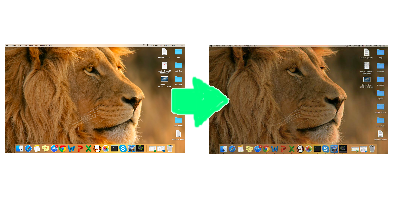
\includegraphics[width=0.5\textwidth]{figs/brightness}
\caption{Brightness of display Change in Level 1}
\label{fig:brightnessChange}
\end{figure}

The way could map the bad posture behaviour and a detectable effect without making a negative user experience. However, the non-informative feedback has two primary limitations. First, the users may simply adapt to the stimuli. Second, there is no explanation for the delivery of the feedback and the user might be confused about where the problem from. The first limitation could be overcome by providing other feedback with stronger intervention extent that the users could no longer easily ignore or adapt to, and the second limitation would require some informative feedback methods to be delivered in the mean time to overcome. The projectors could produce the animation of an elf (See Figure~\ref{fig:transparent_elf}), which has the abbreviation of \textit{Embedded Live-posture Feedback} on the wall, which show graphical indications about how to improve current posture. The indications would be illustrated in a relaxing tone with high degree of the transparency that decreases the extent of interference. Another method is to provide the spelling suggestions by the mobile device when a target posture is detected and the user is typing. The method presents the keywords related to the user’s current posture and therefore enhance the user’s awareness on it. The system would also switch the presentation of an input letter loceated close to the beginning letter of the keyword for current detected posture in the keyboard into the keyword’ beginning letter, therefor the keyword can be suggested. For examples, the system would suggest ``slouch'' when a user with a slouch posture types “s”, and it would also switch the presented letter as ``s'' even the user typed ”d” actually for the suggestion of ``slouch'' to be presented again. The index of the input letter, presented letter and the spelling suggestion is illustrated in Table~\ref{tab:input_letter_spelling_lvl1}. 

\begin{figure}[h]
\centering
  
\includegraphics[width=0.5\textwidth]{figs/transparent1}
\caption{Sample Animation Illustration Decomposition}
\label{fig:transparent_elf}
\end{figure}

\begin{table}
\centering
\begin{tabular}{l c c l} 
\hline\hline
Condition & Input & Present & Suggestion Word\\
\hline\hline
General & B & B & body\\
  & P/O & P & posture/pain\\
  & H & H & health\\
  & S & S & sit/soreness\\
\hline
Lower back & B & B & back\\
not supported & L/K & L & lower-back\\
  & S & S & spine\\
\hline
 Slouch & B & B & back\\
  & S/A & S & spine/slouch\\
\hline
 Stationary & M & M & move\\
  & S & S & shake\\
  & W & W & wave\\
 (specific region) & A & A & arm\\
  & L & L & Leg\\ 
  & T & T & trunk\\
  & H/G & H & head\\
\hline
Bad viewing height/ & D & D & distance\\
distance  & E/W & E & eye/eye-care\\
  & N/M & N & neck/neck-tilt\\
  & S & S & sight\\
  & T & T & tilt\\
  & V & V & viewing-height\\
\hline
Cross Leg & C & C & cross-leg\\
  & L & L & leg\\
\hline\hline
\end{tabular}
\caption{Index of Input, Presented Letter, and Spelling Suggestions in Level 1}
\label{tab:input_letter_spelling_lvl1}
\end{table}

In addition, there are some feedback methods targeting a particular posture. The projector would produce the shadow on the top side of the furniture for a high viewing height posture, which is an implication showing the user is currently tilting his/her head and looking from bottomside up (See Figure~\ref{fig:hvh}). The colour of the shadow could change from time to time to be more fancy and avoid causing a sense of depression related to the colour of gray scale. The projector could also highlight the edge of the furniture to make the sense that the user is currently close to it to feedback a short viewing distance posture (See Figure~\ref{fig:svd}). 

\begin{figure}[h]
\centering
  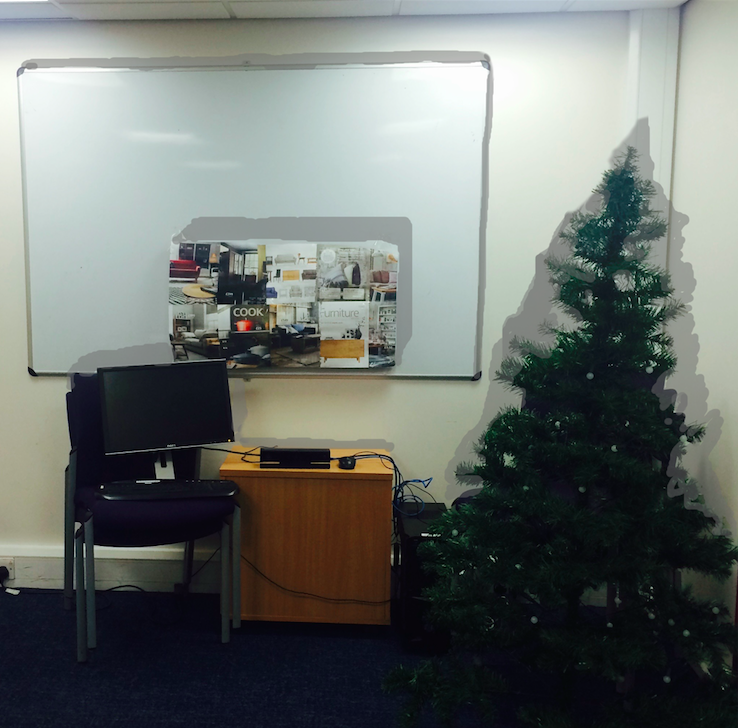
\includegraphics[width=0.5\textwidth]{figs/projector2in1}
\caption{Projector Feedback for High Viewing Height}
\label{fig:hvh}
\end{figure}

\begin{figure}[h]
\centering
  \includegraphics[width=0.5\textwidth]{figs/projector3in1}
\caption{Projector Feedback for Short Viewing Distance}
\label{fig:svd}
\end{figure}

To conclude, the design rationale behind the feedback in this level is to be noticeable but cause the least interference to the activities that the users are engaging in, and the provide a user experience which is not flat or annoying. The feedback methods in the level are summarised in Table~\ref{tab:feedback_model_lvl1}.

\begin{table}[h]
\centering
\begin{tabular}{l l l} 
\hline\hline
 Condition & TV + Mobile Devices & Projectors\\
\hline\hline
 &1. Decrease the volume & 1. Slightly flicker\\
Any bad posture &2. Dim the displays & \\
&3. Switch input letter and & \\
 & \ \ \ \ provide spelling suggestion & \\
\hline
 &  & 1. Provide animation \\
 & &2. High viewing height: \\
 && \ \ \ \ Project shadow for furniture\\
Specific posture&1. Switch input letter and & 3. Low viewing height:\\
  & \ \ \ \ provide spelling suggestion& \ \ \ \ Project shadow for furniture\\
  & & 4. Close viewing distance:\\
  & &\ \ \ \ Highlight furniture edge\\
\hline\hline
\end{tabular}
\caption{Feedback Model in Level 1}
\label{tab:feedback_model_lvl1}
\end{table}

\section{Level 2 : Subtle to Obtrusive}
The intervention extent of feedback would increase if the effect of the feedback in subtle level did show. The amplitudes of the methods used in level 1 would be increased and some new candidate methods in this level. The methods can be classified into two groups according to their targeting posture type, which are general and specific. A general feedback is provided using the projector to make an angle and a devil clock on the wall respectively counting the total duration that the user has bad postures and good postures (See Figure~\ref{fig:adc}). On the other hand, the mobile devices also support two feedback methods for general target postures. The first method is to increase the presentation priority of posture-related news or research on the social media, which could increase the possibility for the users to receive the related information and be aware of the need for posture improvement. The second method is to switch the original ring tone for the mobile phone to the theme song of the system. Both the melody and the lyrics could be helpful on reminding the users to improve the posture. 

\begin{figure}[h]
\centering
  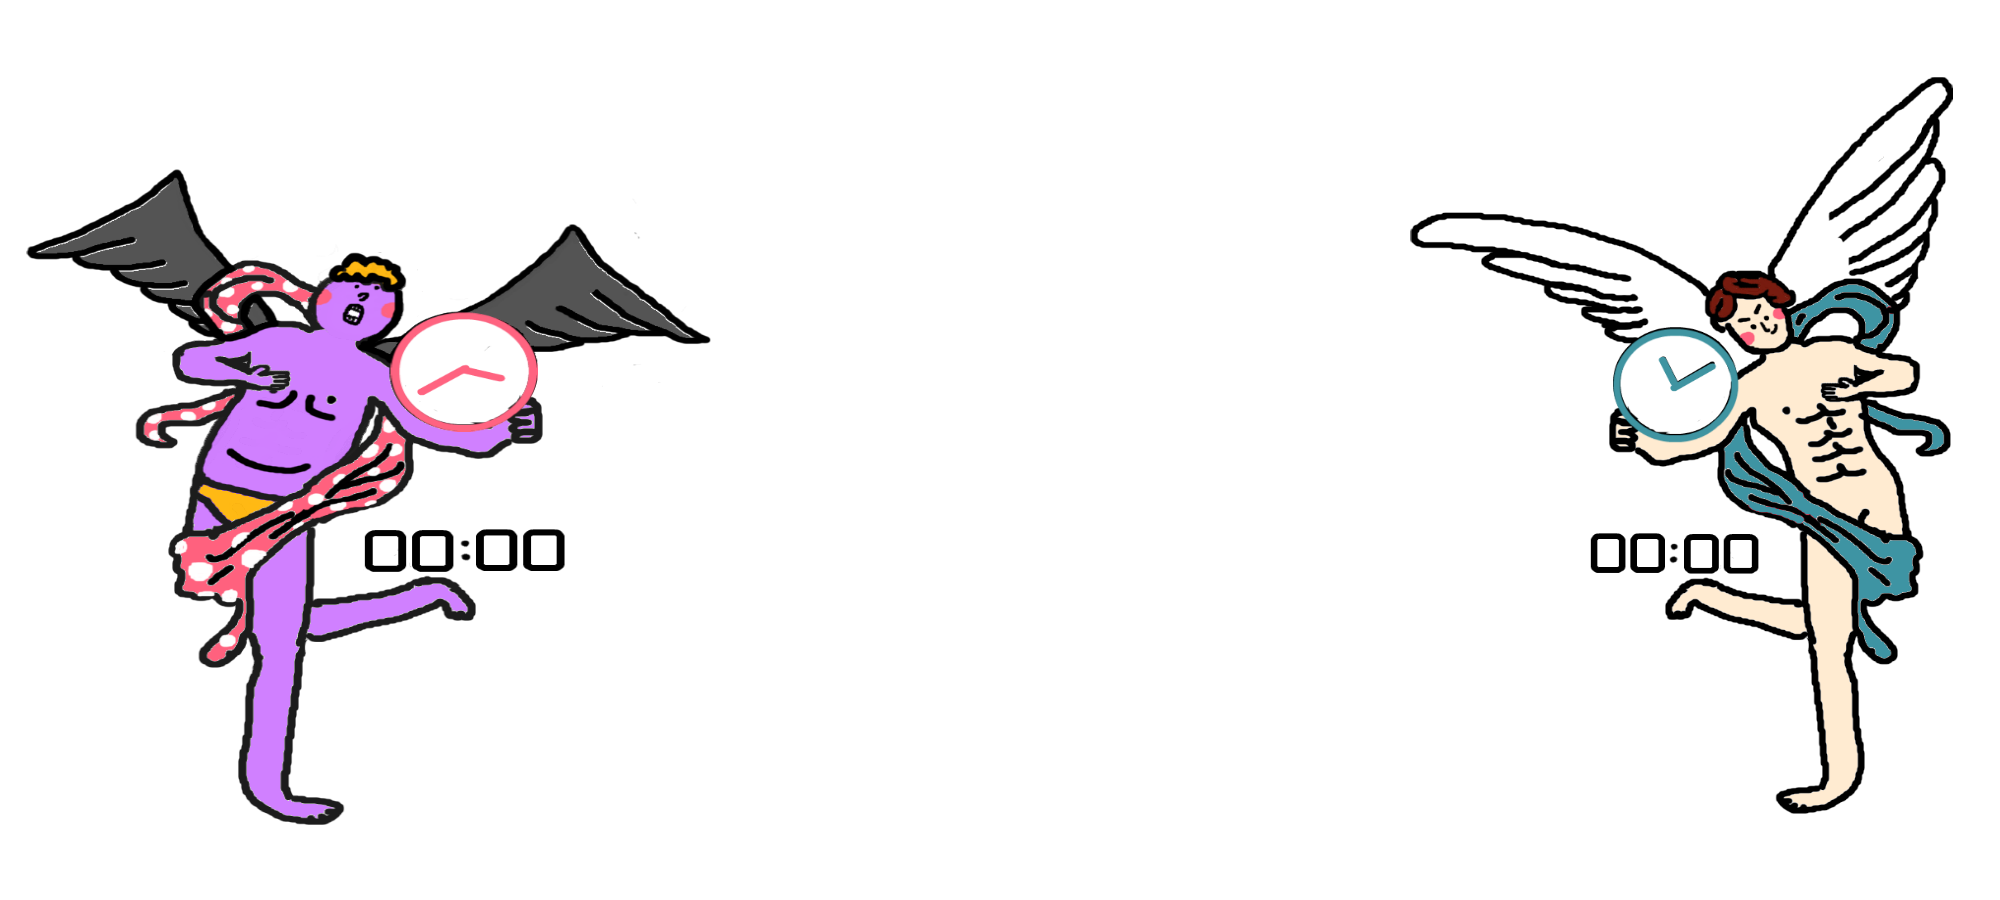
\includegraphics[width=0.5\textwidth]{figs/ad}
\caption{Angel and Devil Clock Feedback}
\label{fig:adc}
\end{figure}

For the feedback targeting a specific posture, the projector would make the effect as there is a starring sky on the ceiling, with shooting stars falling onto the floor to lead the sight of the users downwards for a high-viewing height posture, the starring sky would then fade away while some flowers grows up from the floor. The projector would also feedback to a low-viewing height posture by making some figures of the nestlings slowly fly upwards from the bush on the floor to lead the sight of the users upwards.

For the slouch or lower back not supported posture, the projector could provided the illusion that the room is slightly rotated against the x-axis to simulate the detected posture, by projecting the transformed picture in the same scale of the room. Same techniques could be used to provide feedback to a cross-leg posture, which is to make an illusion that the room rotated against the z-axis and the room’s centre of gravity perceived as moving towards to the opposite side of the upper leg. The sense of imbalance could make the user to put the upper leg down to try to make the sense of balance to the room returns.

If a stationary posture were detected, the projector would create the effect which looks like the furniture in the room is shaking and the dusts accumulated on the top of it are falling down, which implies that the user has kept stationary for too long even the dusts could be accumulated. The mobile device, on the other hand, would feedback to a short viewing distance posture by delivering a GPS-like notification to indicate the user how far he/she currently is from his/her supposed “destination” for a user with the posture.

There are some methods that could be applied to any target posture. First, the projectors could project a skeleton structure onto the wall, with the constrained joints due to the user’s current posture highlighted by different colour, bigger size, and flicker effect. Second, if the user were using an interface containing many words on the mobile device, the letters that consist the keyword related to the current posture would be subsequently highlighted. Third, the social media would be set to recommend some news or research related to the users current posture, helping the user to get more understanding about the impact it might cause and the need on improving it. Forth, an application could be developed on the mobile devices in the form of a messenger. The system would deliver the information, illustrated by animation with or without a voice effect, of current posture, and enable the interaction. 

The candidate methods can cooperate with each other to make the effect of the system more significant. The methods proposed in this level is summarised in Table~\ref{tab:feedback_model_lvl2}. 

\begin{table}
\centering
\begin{tabular}{l l l l} 
\hline\hline
 Condition && TV / Mobile Devices & Projectors\\
\hline\hline
General & &1. Decrease volume & 1. Flicker\\
 & &2. Dim displays &2. Angle clock / devil clock\\
& &3. Reset ring tone &\\
 & &4. Reset screen saver &\\
\hline
Specific & Common &1. Auto correct
inputs  & 1. animation presentation\\  
 & & 2. Recommend related news  & 2. animation guide\\
 & & 3. Send messages & \\
 & & (visual+audio+touch) &\\
 & & 4. Highlight keyword in text &\\
 & & 5. Skeleton impact highlight &\\
\hline
 & Viewing & & High viewing height:\\
 & height & & 1. shadows on the bottom\\
 & & & 2. starring sky animation\\
 & & & Low viewing height:\\
& & & 1. shadows on the top\\
 & & & 2. nestlings animation\\
\hline
&viewing & Deliver GPS notification &  Highlight and widen\\
& distance & & furniture edge\\
\hline
& Lower & & Illusions for room\\
 & back & & rotated against x-axis\\
\hline
& Slouch & & illusions for room\\
& & &  bent from x-axis\\
\hline
& Leg &&  Illusions for room\\
& crossed &&  rotated against z-axis\\
\hline
& Stationary & & Illusion for furniture\\
&&& shaking and dusts falling\\
\hline\hline
\end{tabular}
\caption{Feedback Model in Level 2}
\label{tab:feedback_model_lvl2}
\end{table}

\section{Level 3 : Obtrusive}
Some feedback methods in this level are modified using of the methods proposed in the prior levels. For example, the volume of the speakers as well as the brightness for the displays would be increased when a target posture is detected instead of decreased and dimmed. The design rationale behind this is to make the user not simply able to detect the change, but under higher stimuli as well. Also, the system would automatically correct some words beginning with the letter for the keyword of current detected target posture rather than simply suggest it, which makes the message less likely to be ignored. The index that indicates the details of the functions can be seen in Table~\ref{tab:feedback_model_lvl2}.


The other modifications from the previous methods include switching the mobile into outdoor mode, and the ring tone becoming the voice command for current posture improvement; making the projected shadow of furniture for a low viewing height or high viewing height posture dynamic, which can extends upwards or downwards; and the highlighted furniture edge feedback for the short viewing distance posture would flicker and wave.

There are also many new feedback methods proposed. First, the users would be asked by the system to present that they would make efforts on their posture improvement when they firstly use the system. The picture taken by the Kinect when the user mad promise could be projected onto the wall in this level, using the rationale of cognitive dissonance to remind the users to keep their behaviour consistent. They would tend to change the later action (having a bad posture) according to the prior action (making promise to have good posture for the goods of health) to avoid the anxiety caused by the cognitive dissonance. 

Secondly, a method inspired by the design of Half Room~\cite{half_room} (See Figure~\ref{fig:halfroom}) would be integrated with the feedback for cross-leg, lower back not supported and slouch posture. The position and the orientation of the half room are modified for each posture individually. This is for using the half room’s design rationale of anxiety avoidance and curiosity about the extending, to push the users to change current posture. For example, when there is a lower back not supportive posture, the half room picture would be projected and perceived parallel to the body, in which the user would change the posture to avoid the anxiety caused by the alignment and explore what could be shown in the blank.

\begin{figure}[h]
\centering
  \includegraphics[width=0.5\textwidth]{figs/halfroom}
\caption{Weighting for audio forms}
\label{fig:halfroom}
\end{figure}

Thirdly, some 3D objects could be projected on the area close to the display to make a crowding sense for user having a short viewing distance posture. At last, the printer could automatically colour print the picture of the user with his/her current posture, along with the description of the duration of current posture, the impact it might cause to the body, and the relevant research on it. It could be a powerful method to instruct the user about what should be understood about the user. 
The cooperation between multiple methods in the level is presented in Table~\ref{tab:feedback_model_lvl3}. 

\begin{table}
\centering
\begin{tabular}{l l l l} 
\hline\hline
 Condition && TV / Mobile Devices & Projectors\\
\hline\hline
General & &1. Decrease volume & 1. Flicker\\
 & &2. Dim displays &2. Angle clock / devil clock\\
& &3. Reset ring tone &3. project promising picture\\
 & &4. Reset screen saver &\\
\hline
Specific & Common &1. Auto correct
inputs  &1. animation presentation\\  
 & &2. Recommend related news  & 2. animation guide\\
 & &3.Send messages & \\
 & &  (visual+audio+touch) &\\
 & &4. Highlight keyword in text &\\
&&  5. elf reminder on &\\
& &  background/browser homepage & \\
& &6. Color print & \\
& &  current pics with &\\
&&  description &\\
& &7. Reser ring tone &\\
& & using voice command & \\
& & 8. Skeleton impact highlight& \\
\hline
 & Viewing & & High viewing height:\\
 & height & & 1. shadows on the bottom\\
 & & & 2. starring sky animation\\
 & & & 3. half room\\
 & & & Low viewing height:\\
& & & 1. shadows on the top\\
 & & & 2. nestlings animation\\
 & & & 3. half room\\
\hline
&Viewing & Deliver GPS notification &1. Highlight and widen\\
& distance & &  furniture edge\\
& & & 2. Make 3D objects full\\ 
\hline
& Lower & &1. Illusions for room\\
 & back & &  rotated against x-axis\\
 & & & 2. Half room\\
\hline
& Slouch & &1. Illusions for room\\
& & &  bent from x-axis\\
 & & & 2. Half room\\
\hline
& Leg && 1. Illusions for room\\
& crossed &&  rotated against z-axis\\
 & & & 2. Half room\\
\hline
& Stationary & & illusion for furniture\\
&&& shaking and dusts\\
&&& falling\\
\hline\hline
\end{tabular}
\caption{Feedback Model in Level 3}
\label{tab:feedback_model_lvl3}
\end{table}

\section{Summary}
The model aims at discussing various ways to provide feedback to the detected postures. 10 candidate methods are proposed in level 1, while 20 methods are proposed in level 2 and 33 methods in level 3. The structure of the model is illustrated in Figure~\ref{fig:feedback_model_2}. The colours are used to encode the targeting posture types, and the presentation of the gradient background of a feedback method indicates that the intervention extent of the method would become increase if the improvement of the target posture were not observed. 

\begin{figure}[h]
\centering
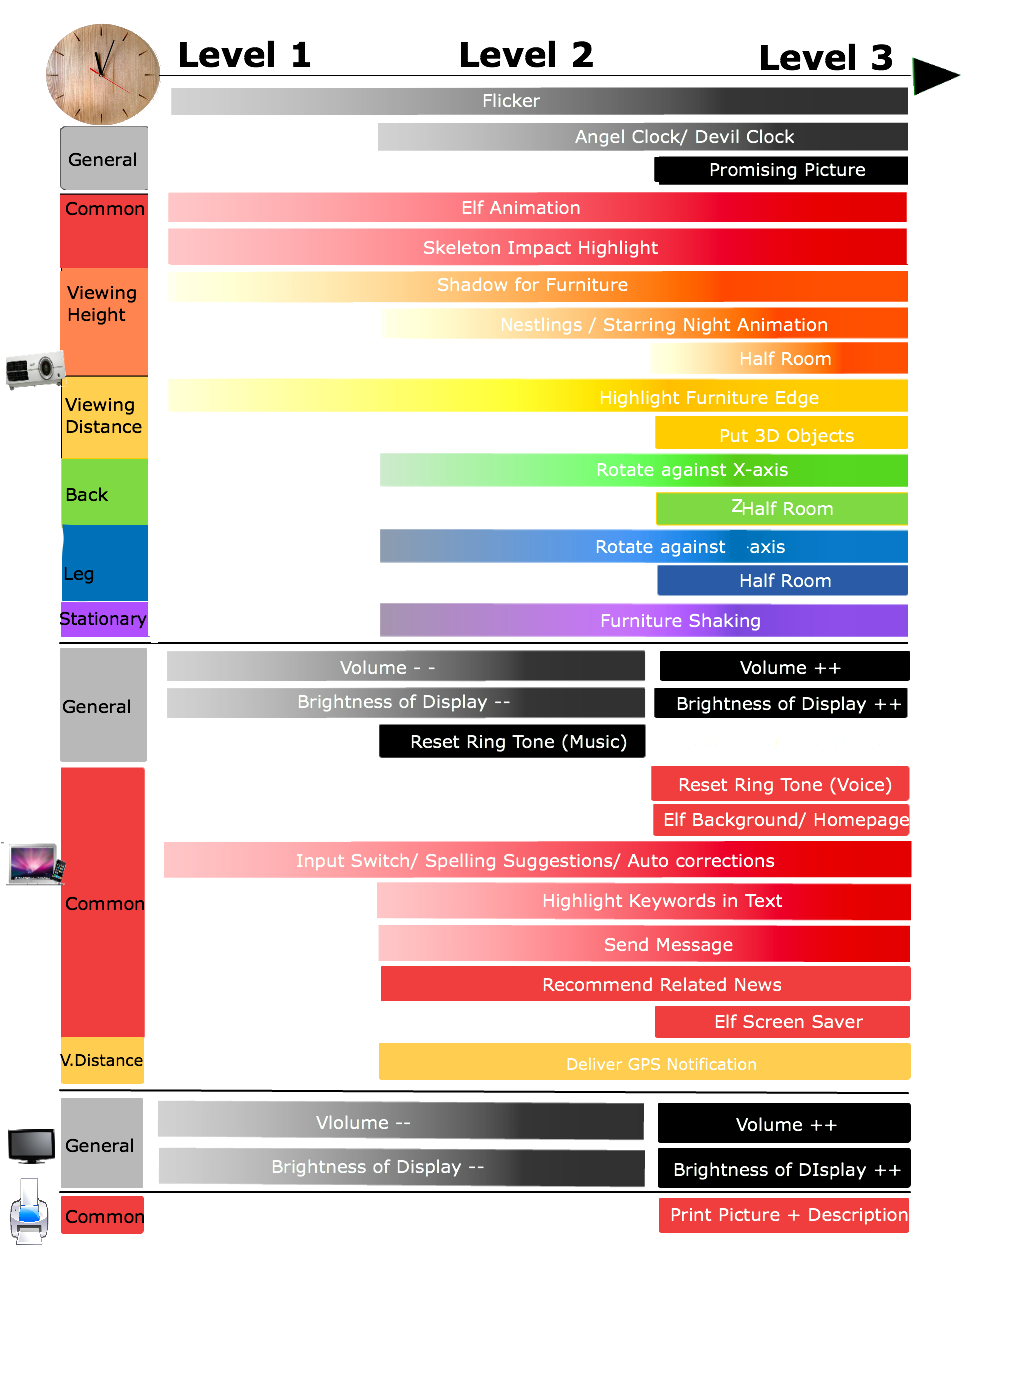
\includegraphics[width=1\textwidth]{figs/feedbackmodel2}
\caption{Feedback Model}
\label{fig:feedback_model_2}
\end{figure}

\chapter{User Study}

\section{Objective}
\section{Objective}
The objective of the study was to build the posture classification model, analyse the posture behaviour patterns in two scenarios, and investigate the perspectives to the issues related to the design of the system.

\section{Method}
\subsection{Posture Measurement}
The study had three sections. In the first section, the postures would be measured. A proper posture would be assessed in the beginning of this section to set the baseline. Following, The participants would be asked to have a particular posture type, such as slouch, given a degree of freedom for them to interpret the posture by their usual way. The step would be repeated for four times until the target postures including cross-legs, slouch, lower back not supported, and stationary were measured. Each measurement would last for 3 minutes, but the participant would not be informed in advance. They were encouraged to relax and do their chosen relaxing activity, such as watching TV or surfing the internet on their mobile devices. This aims at simulating the normal conditions that the participants engaged in the VTDs related activities with the target unhealthy postures.

A Kinect would be placed right in front of where the participants sit to record the positions of 25 joints in the body. A digital video (DV) would videotape from the side. Each participant would be asked to have all postures in different order to balance a potential carry-over effect. The balance method follows the design of Latin square. The participants would be randomly assigned into four groups and their postures would be observed following the order presented in Table 4.1. Generally, there would be the rest time for one minute between two trials, which could be extended if needed. A Likert five-point scale would be applied during the rest time to get the subjective information about the degree of relax and the degree of shoulder, neck, and spine comfort (namely, discomfort) the participants felt when they were having the tested posture. If a participant reported discomfort in any part of the body due to the posture, a following question would be asked to clarify the sense by giving multiple choices including pain, soreness, and tightness. The subjective judgement for current viewing height and the degree of comfort for current viewing height would also be investigated as the criteria for a low-viewing height posture could be relatively vague. 

\begin{table}[ht]
\centering
\begin{tabular}{c c c c c}
Group&Posture1&Posture2&Posture3&Posture4 \\
\hline
Group1&leg crossed&lower back&slouch&stationary \\
Group2&lower back&leg crossed&stationary&slouch \\
Group3&slouch&stationary&leg crossed&stationary \\
Group4&stationary&slouch&lower back&leg crossed \\ [1ex]
\hline
\end{tabular}
\label{table:nonlin}
\caption{Order of the posture measurement for different groups}
\end{table}

\subsection{Scenario Observation}
In the second section, the behaviour pattern the participants had when they were engaging in the VDT activities would be observed. The participants were randomly assigned into two groups. Participants in the first group would watch their chosen videos on TV, and those in the other group would use their own mobile device freely. The activities for the two groups all lasted for 15 minutes. Some further information would be investigated after the activities, which included the subjective cognition for the degree of relax when doing the prior activity, and the similarity between the behaviours of doing the activity in the lab settings and doing the activity in real life.The data which had a low similarity score would be discarded as the data could not reflect the behaviour pattern for the users in real life. The valid data filtered by the question would be used to analyse the frequency of different target postures. The priority among the target postures for being feedbacked would be decided by the occurrence rate and the degree of discomfort for each posture.

\subsection{Interview}
The aims of the section was to gather more information about the posture pattern for each participant by an interview. The participant would be asked about their:

\begin{enumerate}
\item past musculoskeletal disorder history
\item musculoskeletal discomfort in the past three months and the subjective explanation for it
\item subjective evaluation to the overall posture pattern of themselves
\item awareness of bad postures with respect to the timing and the extend
\item effort had been made to improve postures with respect to the methods, durations, and results
\item reasons to improve the postures
\item preference for different feedback methods subject to a home environment.
\item belief for the effective extent of different feedback methods subject to a home environment.
\item preference for different feedback channel subject to a home environment.
\item belief for the effective extent of different feedback channel subject to a home environment.
\end{enumerate}

\section{Participant}
12 university students aged between 20 and 30, body height between 156 to 172 cm (average = 164.3), with no significant musculoskeletal disorder history.

\section{Material}

\subsection{Experimental apparatus and resources}
The following materials were used to measure the posture, record the procedure, facilitate the scenario observation and the interview, and ask the subjective feelings and perspectives of the participants.

\begin{itemize}
 \item A Microsoft Kinect
 \item A digital video
 \item A television
 \item Tokens
 \item Likert five-point scales:
  \begin{itemize}
   \item degree of relax
   \item degree of neck comfort
   \item degree of shoulder comfort
   \item degree of spine comfort
   \item degree of current viewing height
   \item degree of the similarity between the behaviours in the test condition and normal condition
  \end{itemize}
\end{itemize}

\subsection{Documents for ethics approval}

The ethical considerations of the study were approved by The University Teaching and Research Ethics Committee. The approval letter for the study could be seen in Appendix H. The following sheets were given to the participants to protect their right and ensure they understood the study.

\begin{itemize}
\item Participant Information Sheet (See Appendix~\ref{appendix:information_sheet})
\item Participant Consent Sheet (See Appendix~\ref{appendix:consent_form})
\item Participant Debriefing Form (See Appendix~\ref{appendix:debrief_form})
\end{itemize}

\section{Procedure}
The instructions of the researcher through the study would be standardised to decrease the bias (See Appendix~\ref{appendix:instructions}). At the beginning, the researcher would explain the objectives and the outline of the study and then inform the rights of the participants before asking them to read and sign on the consent form. There should be only one participant to take the experiment at one time to avoid potential confounding variables related to their interaction. A set of postures would be measured in a specific order in the first section of the study. Likert scales would be applied between the measurements of two postures. The behaviour pattern for engaging in an VTD related activity would be recorded in the second section. The subjective cognition for degrees of relax when doing the test activity as well as the similarity between behaviours in the test condition and real-life conditions were also investigated. In the last section, an interview was carried out to understand more information about the posture and posture improvement associated perspectives of the participants before the debriefing procedure. The whole study would last for approximately an hour.

\section{Analysis}
The participants rated their posture appropriateness between 2 to 4 (average = 2.92, standard deviation = 0.79) on a Likert 5-point scale. However, even though the participants believed their posture behaviour are not bad in general, there still are 66 percent of the participants who experienced musculoskeletal discomfort, including back, waist and shoulder soreness, neck and shoulder tightness, and neck, shoulder, spine, and back pain, in the past three months. 88 percent of them contributed at least part of the discomfort to bad postures, in particular to the behaviours related to using computer, such as prolonged sitting when working on the laptop.

As for the bad posture awareness, only 25 percent of the participants reported that they would notice they were having a bad posture before feeling any discomfort. 58.33 percent of the participants said they would find they are having posture when they have experienced the soreness, tightness, pain, or numbness caused by it. 16.67 percent of the participants even would not find their current bad postures until they are about to change to another posture. However, the participants gave an average 3.08 for their bad posture awareness (standard deviation = 0.90)on the 5-point scale. The fact might indicate that they tend to overestimate their awareness on bad postures, but current feedback system could be helpful for improving the awareness.

\subsection{Posture Modelling}
There are some formula rendered by the observation of the target postures. The parameters of the formula would be defined using the data collected from the section one : Posture Measurement. The data from the posture measurement procedure would be used to fit the model and find the optimised parameters. The optimised formula for one posture is defined as a formula which has the highest hit rate among the data of the target posture, and the lowest false alarm rate among the data of the proper posture.

\begin{enumerate}
  \item leg crossed (would use the pictures of the participants instead)
  \begin{itemize}
    \item type 1 \hfill \\
    \[| Y of Left Feet - Y of Right Feet | > a\]
    \[AND\]
    \[ Distance( PositionOf Left Knee - PositionOf Right Knee) > b\]

    \begin{figure}[h]
    \centering
      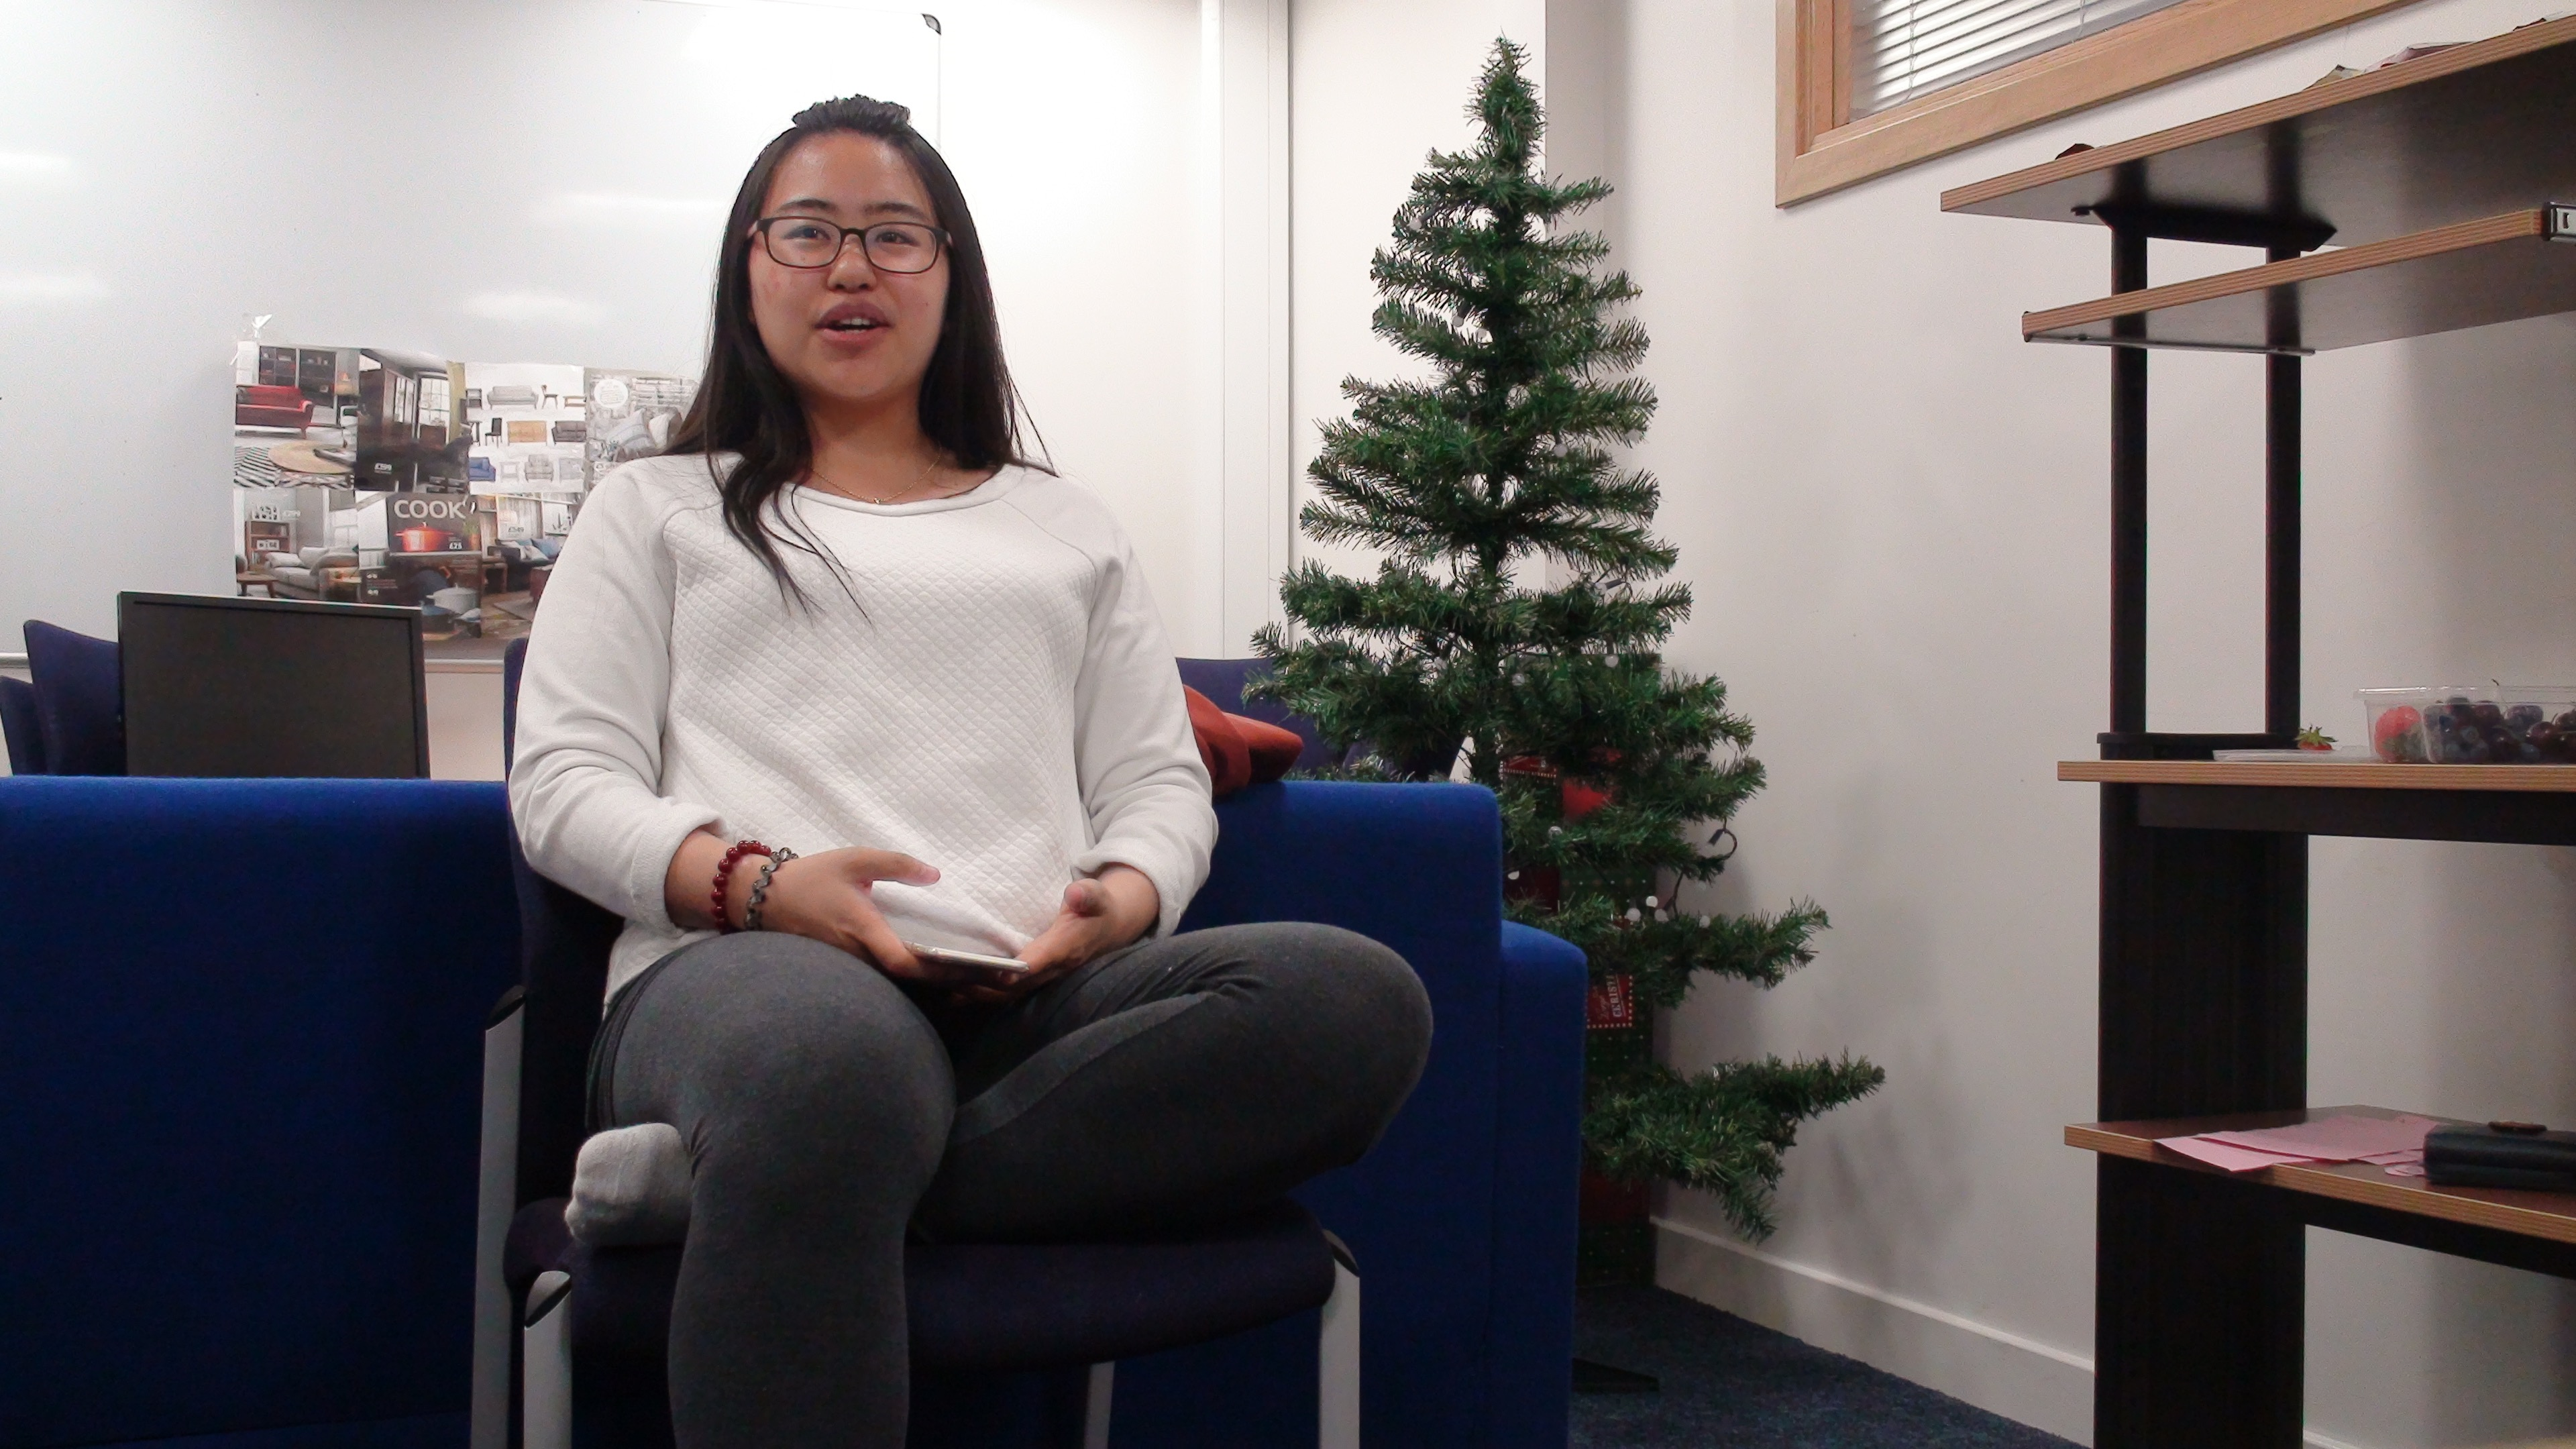
\includegraphics[width=0.5\textwidth]{figs/c1}
    \caption{Leg-Crossed Type 1}
    \end{figure}

    \item type 2 \hfill \\
    \[ ( X of Left Feet - X of Right Feet)* (X of Left Shoulder - X of Right Shoulder) < 0\]
    \[ OR\]
    \[ ( Z of Left Feet - Z of Right Feet)* (Z of Left Shoulder - Z of Right Shoulder) < 0\]\\

    \begin{figure}[h]
    \centering
      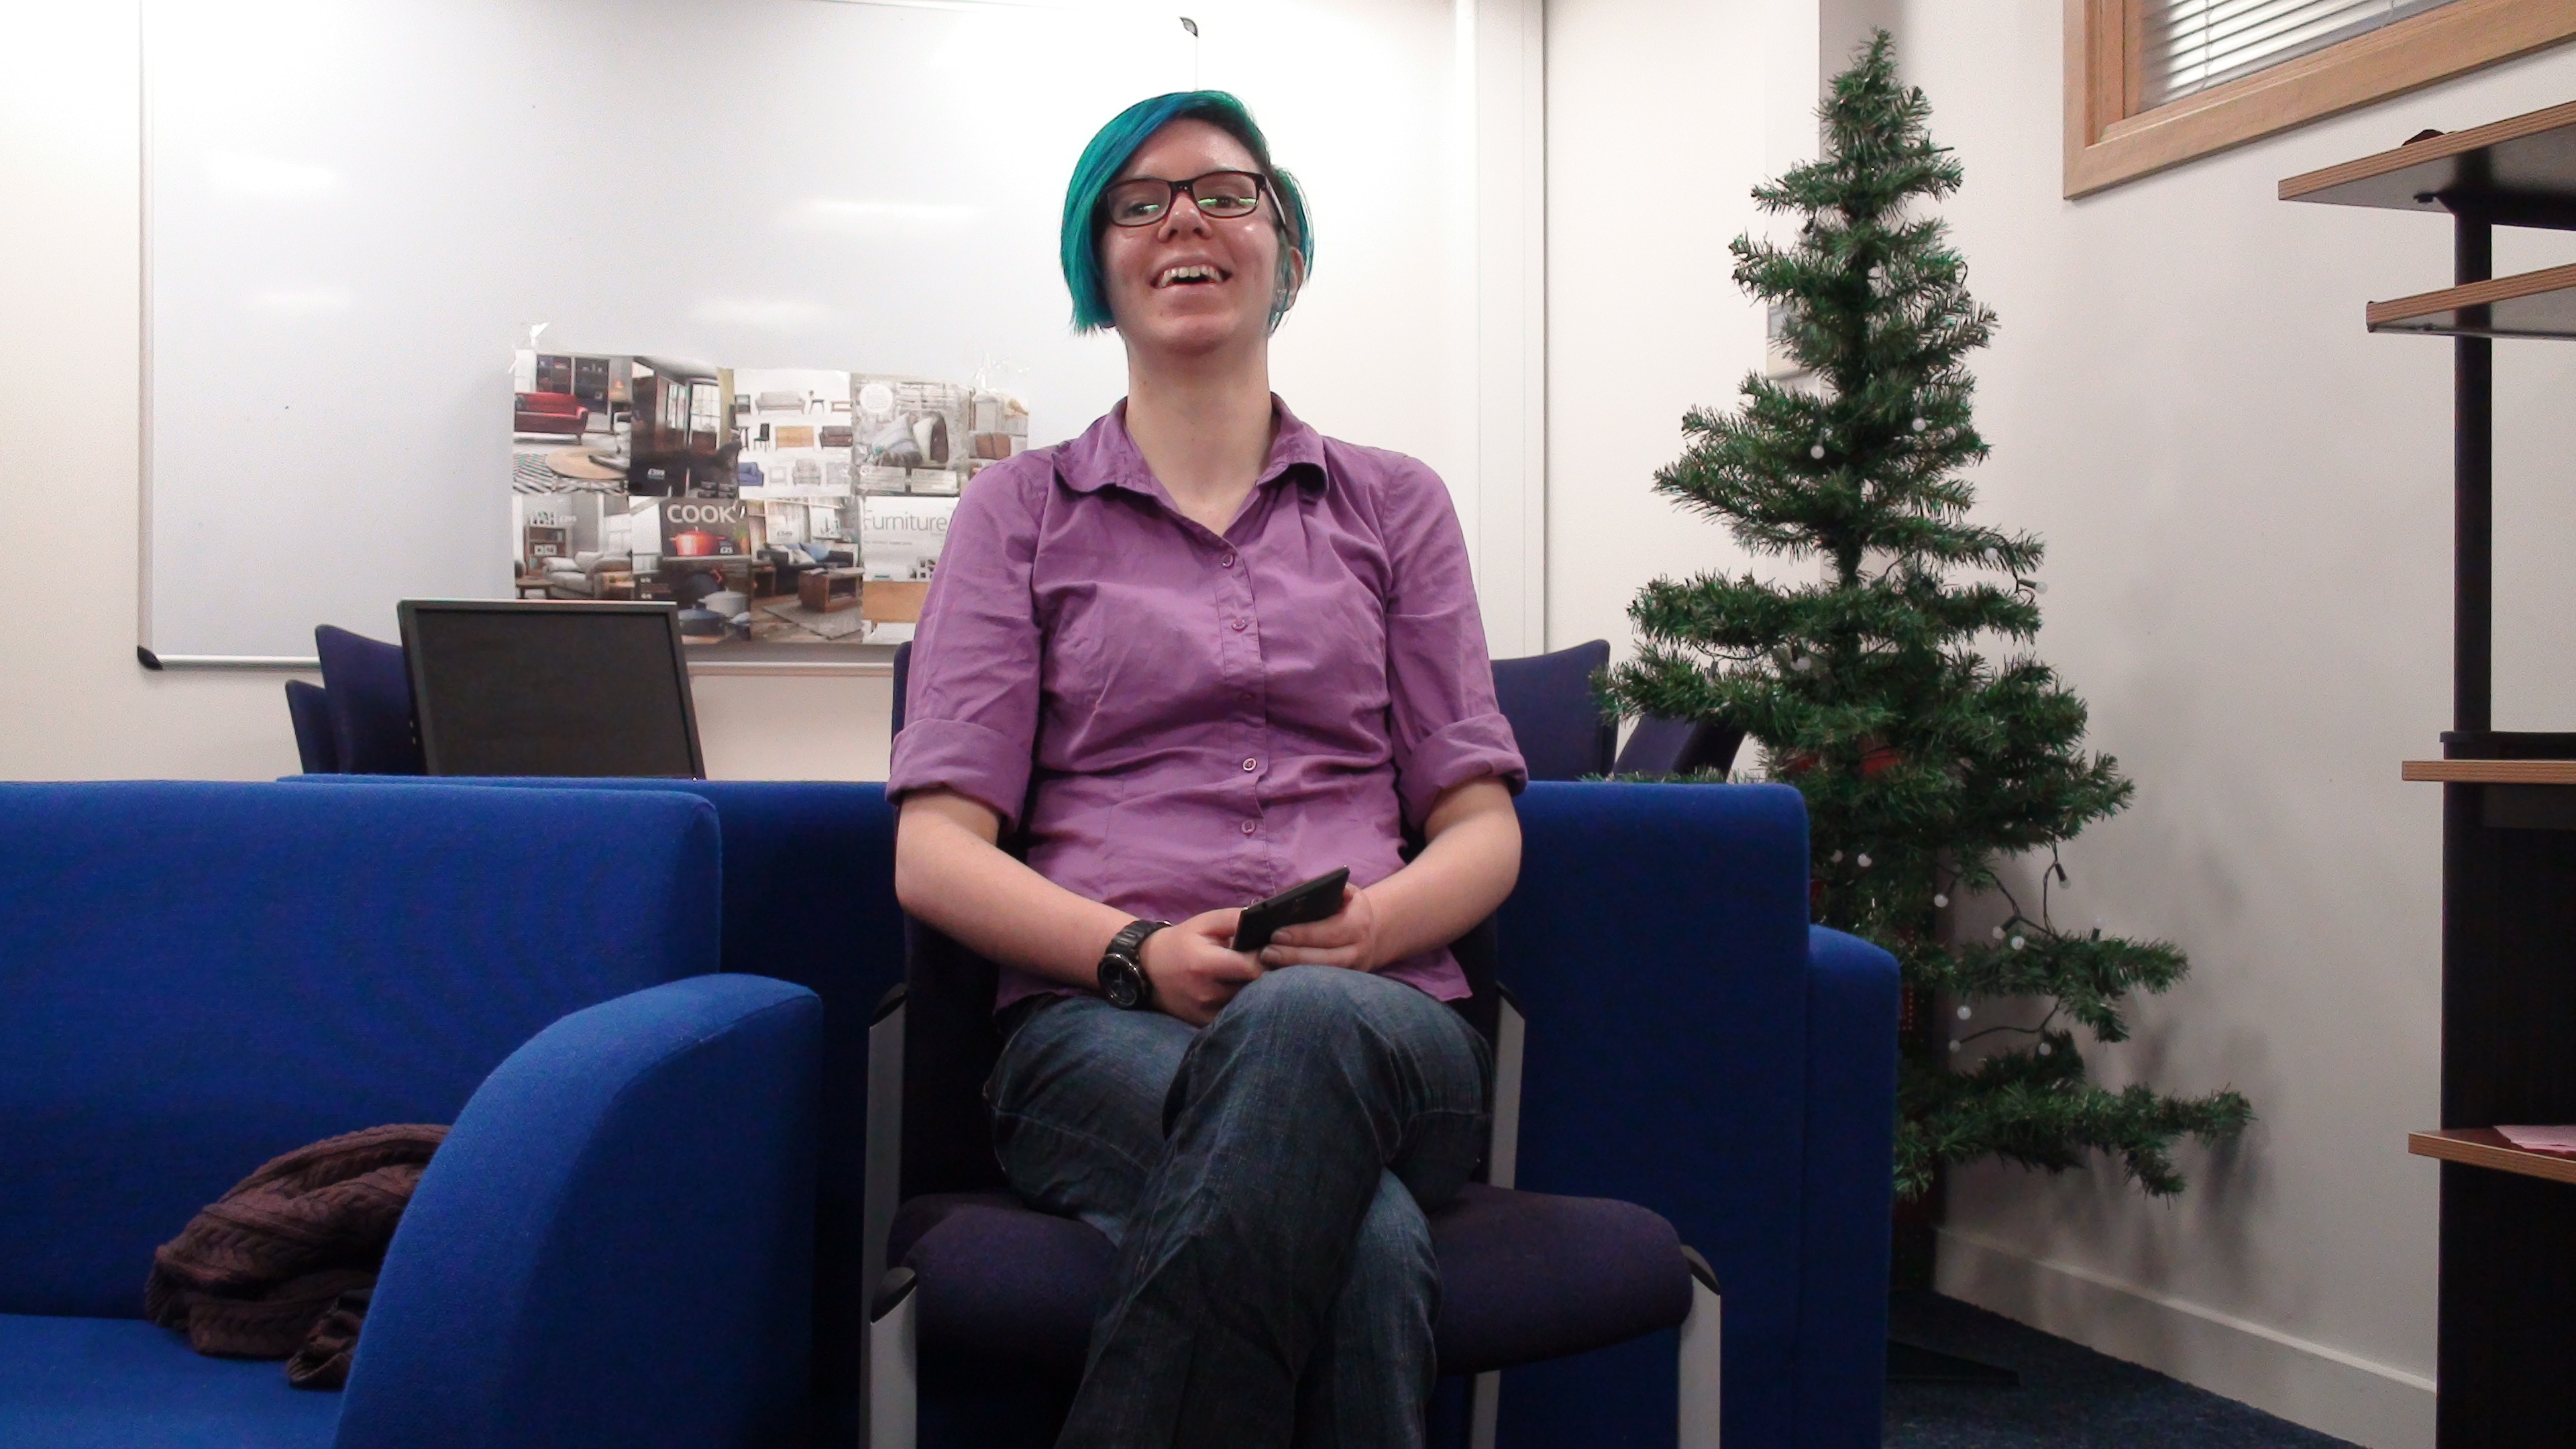
\includegraphics[width=0.5\textwidth]{figs/c2}
    \caption{Leg-Crossed Type 2}
    \end{figure}

    \item type 3 \hfill \\
    \[( ( X of Left Feet - X of Right Feet)* (X of Left knee - X of Right knee) < 0\]
    \[OR\]
    \[ ( Z of Left Feet - Z of Right Feet)* (Z of Left knee - Z of Right knee) < 0)\]
    \[AND\]
    \[ Distance(PositionOf Left Knee - PositionOf Right Knee)> c\]

    \begin{figure}[h]
    \centering
      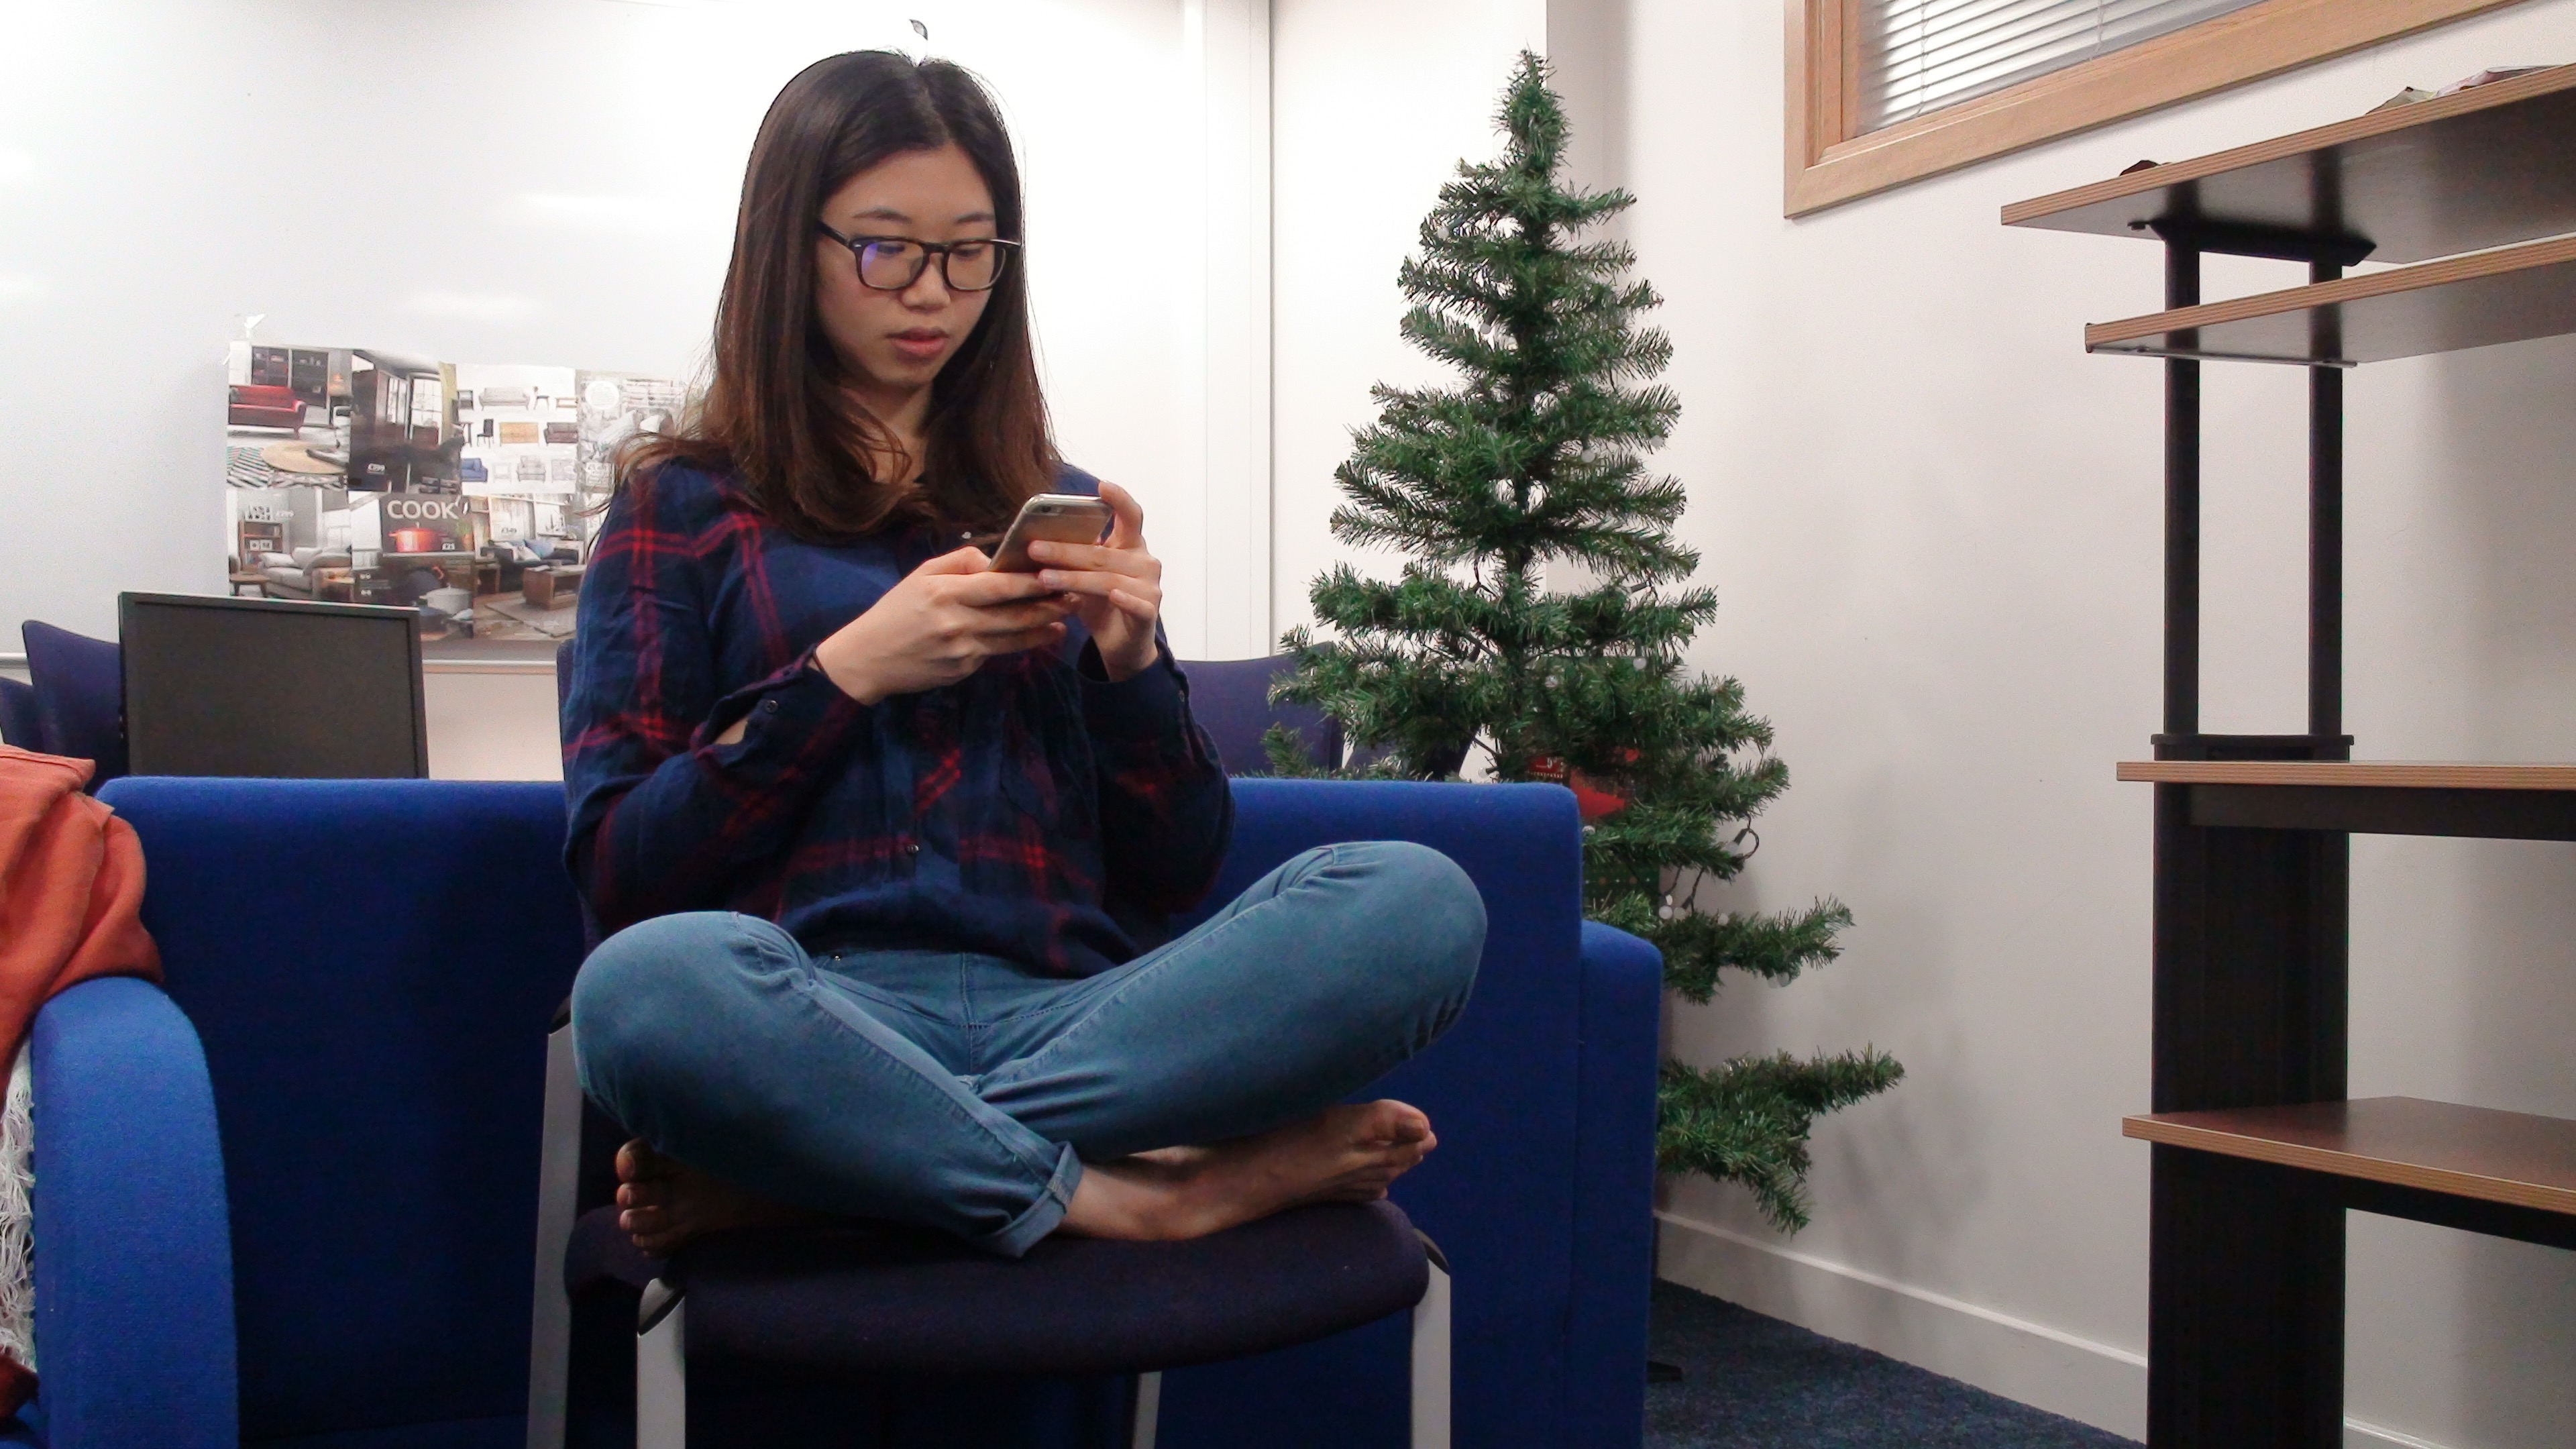
\includegraphics[width=0.5\textwidth]{figs/c3}
    \caption{Leg-Crossed Type 3}
    \end{figure}
  \end{itemize}

  \item lower back not supported \hfill \\
  \[ Z of SpineMid- Z of SpineBase > d\]
  \[ AND\]
  \[ Y of SpineShoulder - Y of SpineBase < e\]
  \begin{figure}[h]
  \centering
    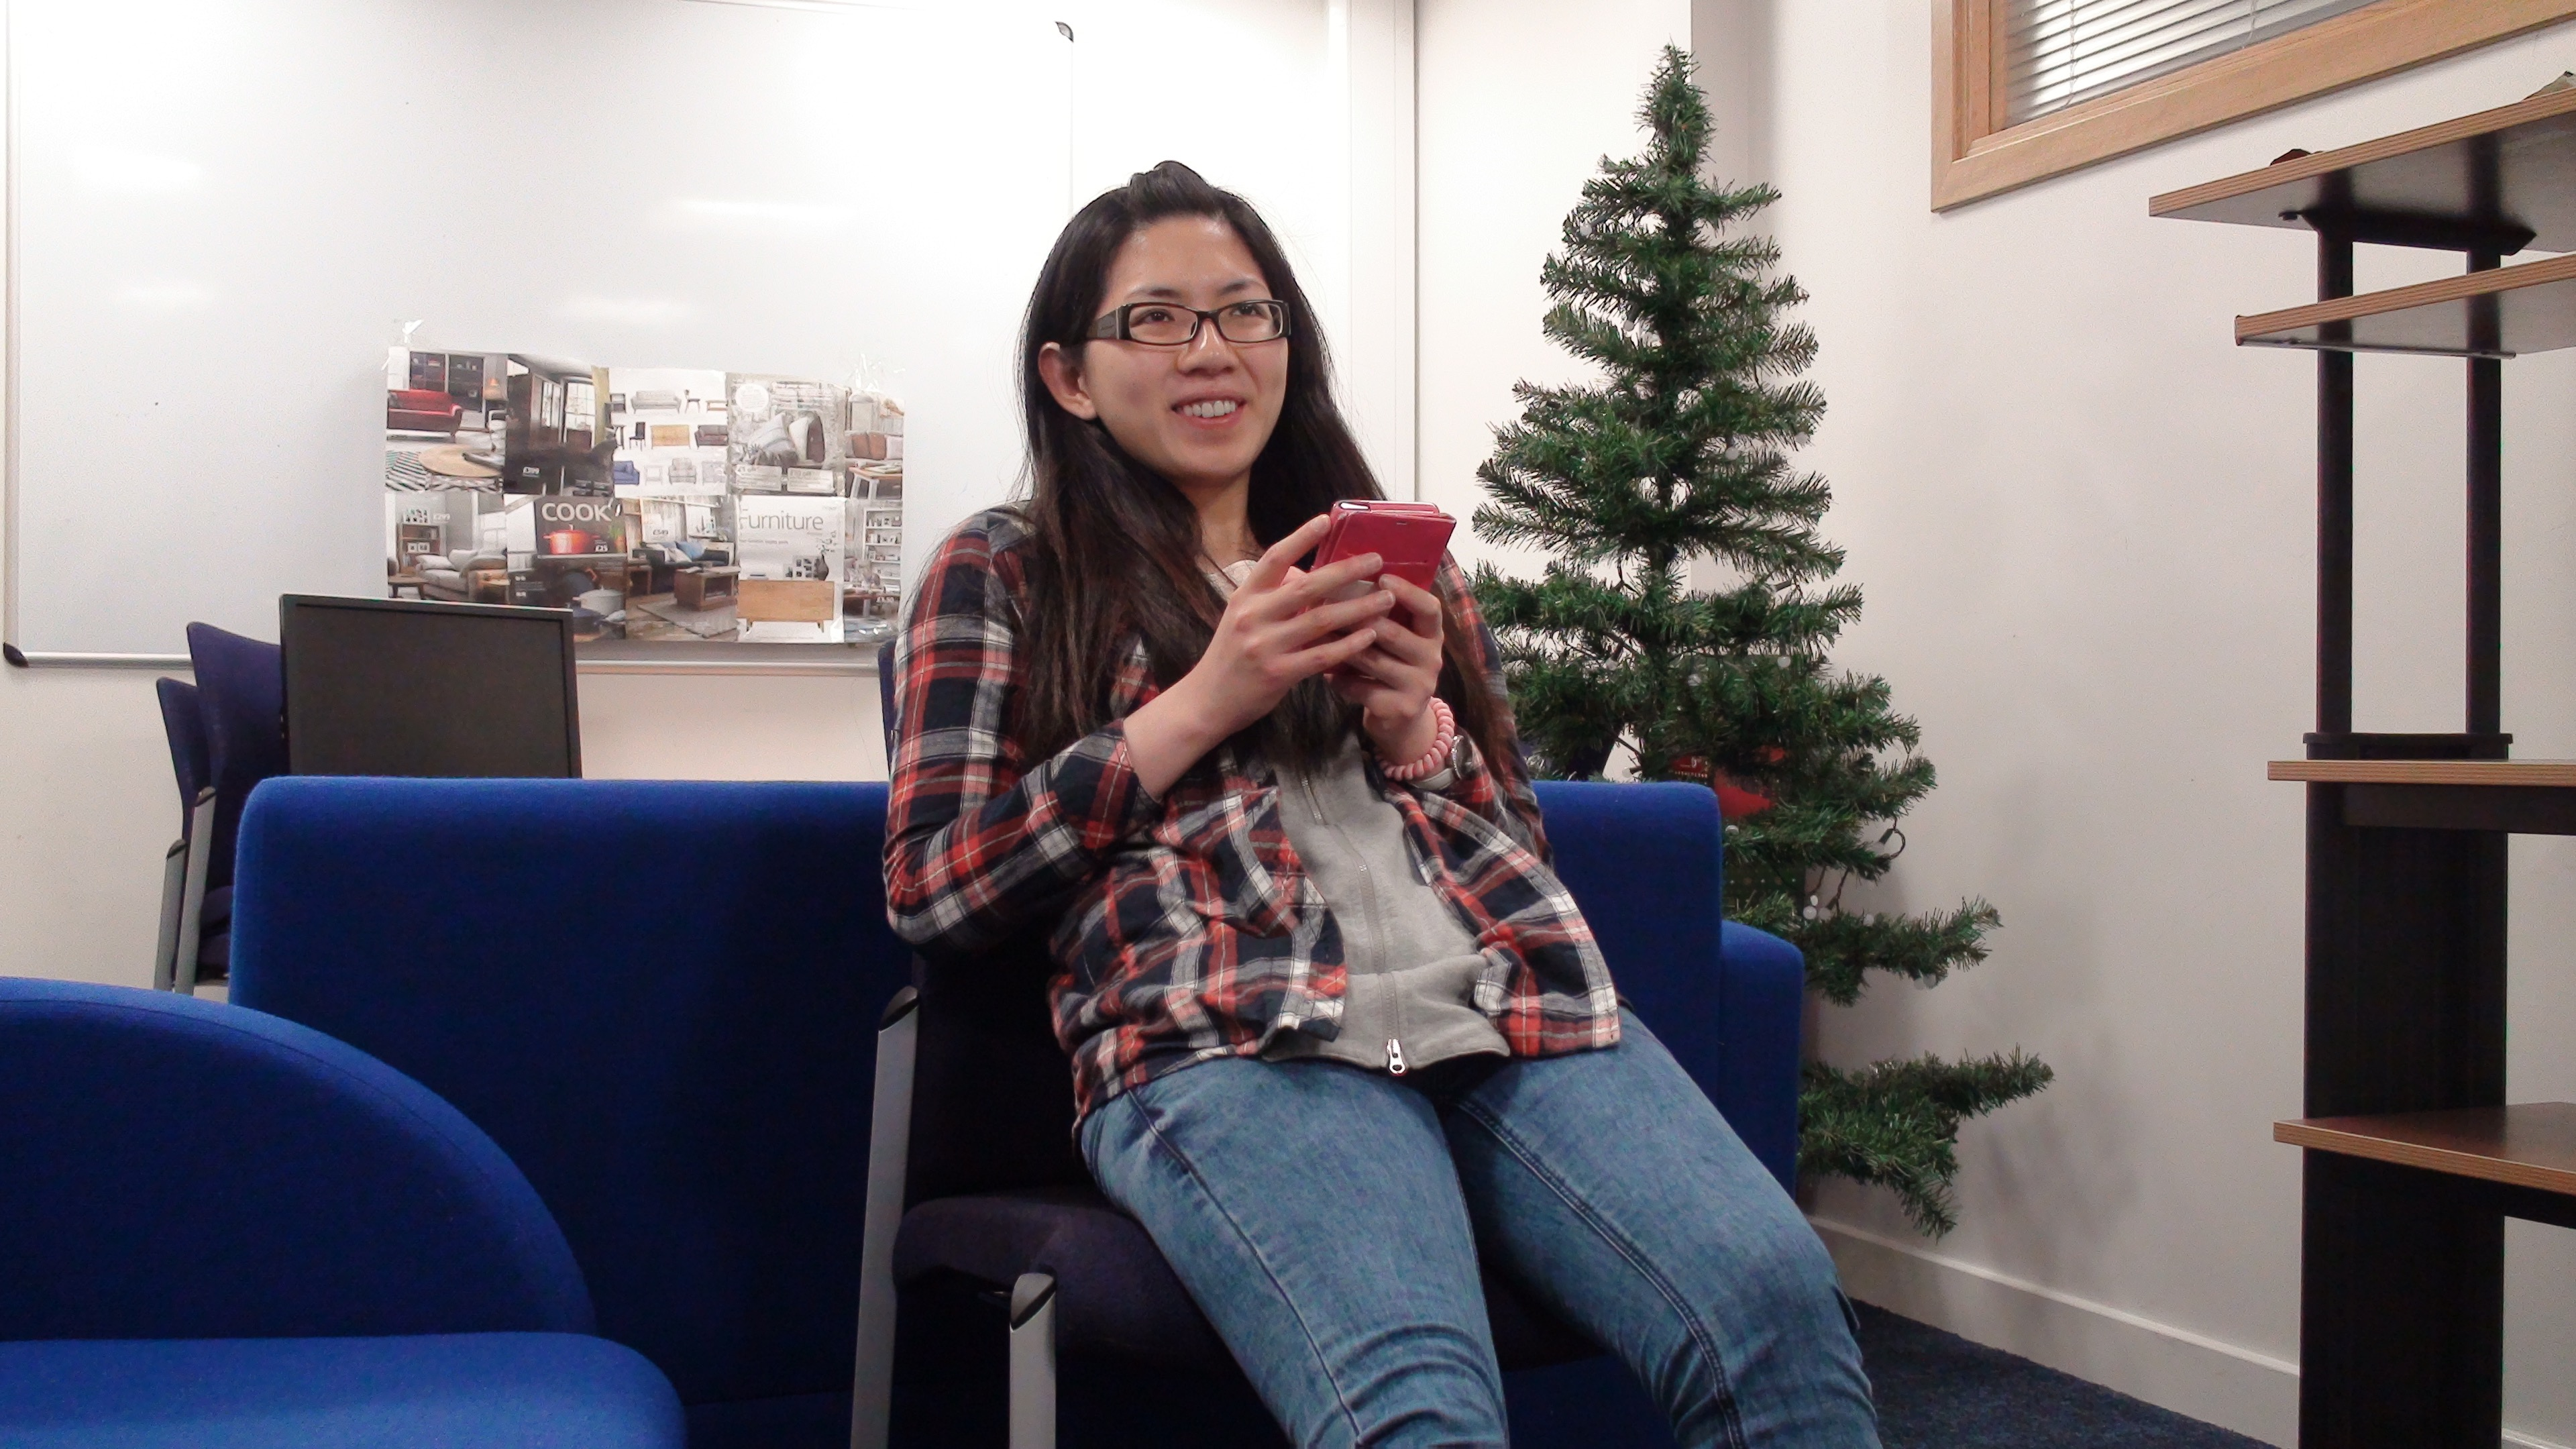
\includegraphics[width=0.5\textwidth]{figs/l1}
  \caption{Lower-Back Not Supported}
  \end{figure}

  *The formula used to classify the lower-back-not-supported posture can adopt position Z of the joints to be its variables, because having this posture should be sitting against the back of sofa and the problem of body orientation should not exist in this condition.

  \item slouch \hfill \\
  \[( Z of SpineMid - Z of SpineBase )*(Z of SpineMid - Z of SpineShoulder )  > 0\]
  \[OR\]
  \[( X of SpineMid - X of SpineBase )*(X of SpineMid - X of SpineShoulder )  > 0\]
  \[OR\]
  \[ Distance(PositionLeftShoulder - PositionLeftHip)< f\]

  \begin{figure}[h]
  \centering
    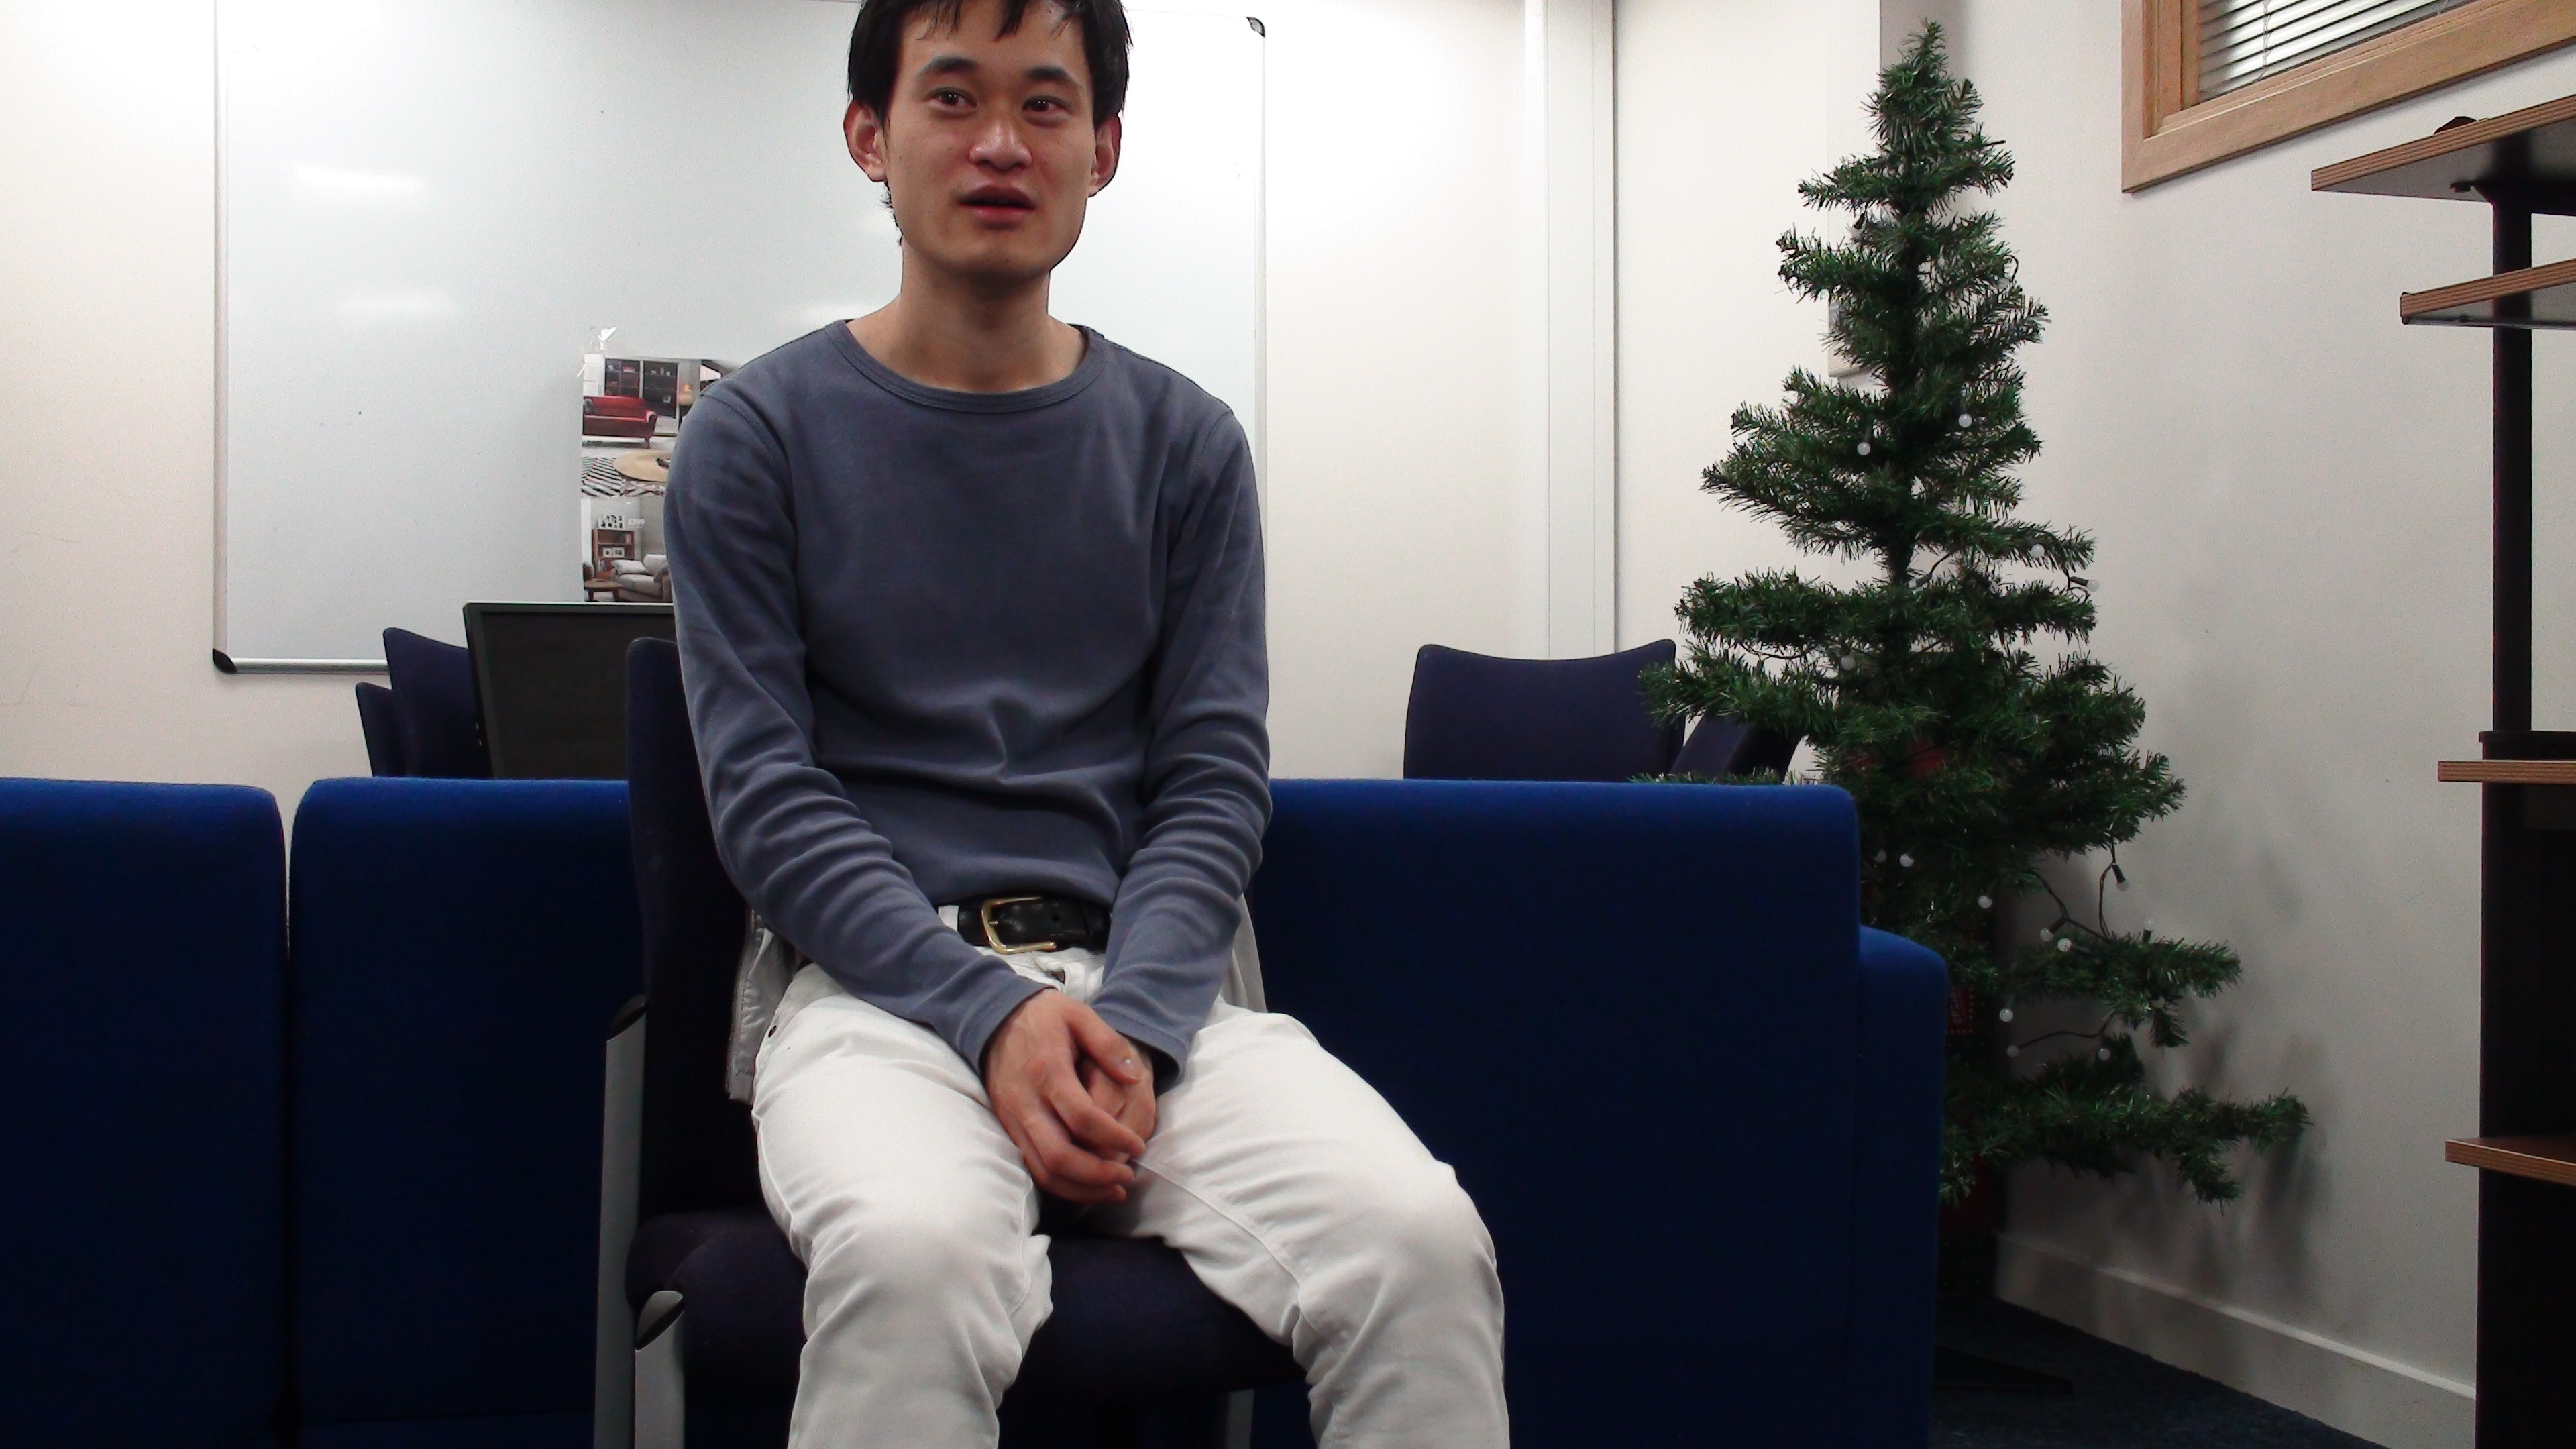
\includegraphics[width=0.5\textwidth]{figs/s1}
  \caption{Slouch}
  \end{figure}

  \item stationary \hfill \\
  *Clean the outliers of the data collected from the stationary posture measurement, and calculate the variance for each joints to define the 99.5 percent confidence interval that the values may vary.
  \item viewing height
  \begin{itemize}
    \item low viewing height
    \[ Y of Head - Y of Neck < g\]
    \[ AND\]
    \[ (Z of Neck - Z of Head > h ) || ( X of Head - X of Neck > i)\]
    \item high viewing height
    \[Y of Head - Y of Neck > j\]
    \[ AND\]
    \[ (Z of Head- Z of Neck > k ) || (X of Neck- X of Head > l)\]
    \begin{figure}[h]
    \centering
      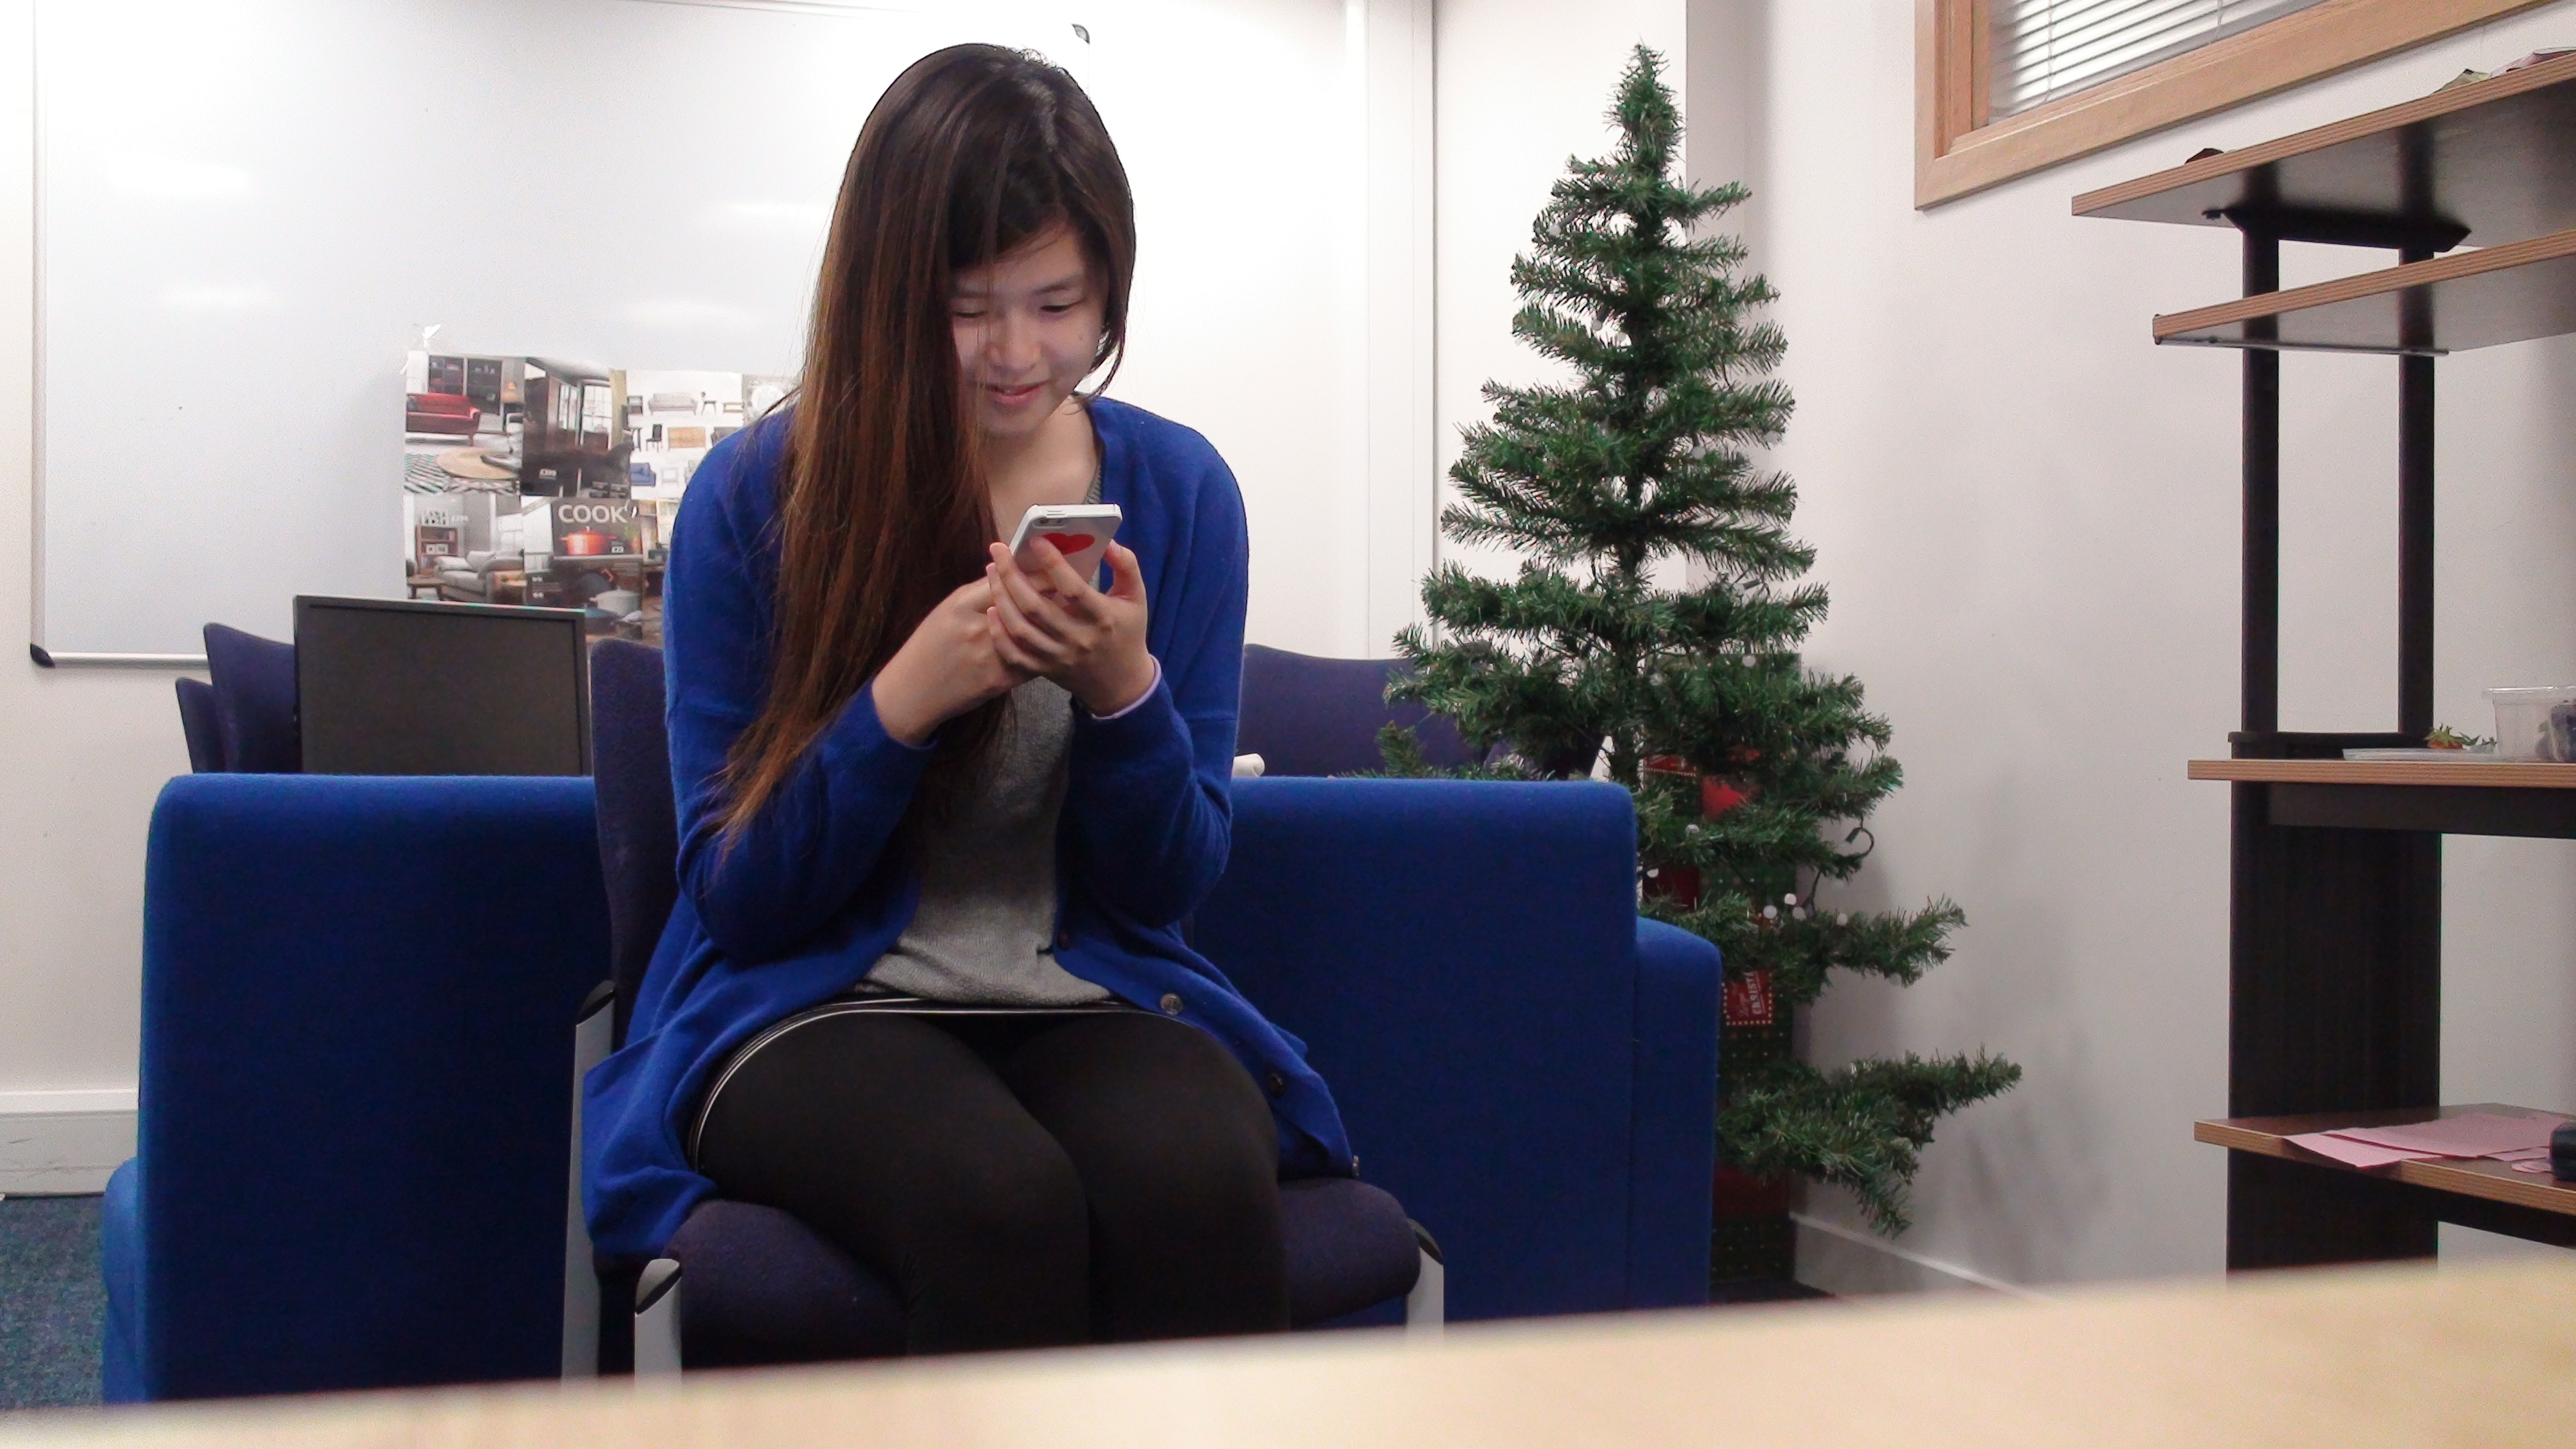
\includegraphics[width=0.5\textwidth]{figs/lh1}
    \caption{Low Viewing Height}
    \end{figure}
  \end{itemize}
\end{enumerate}

\subsection{Priority of Posture Feedback}
The regulation priority among the target postures is determined by both subjective reports in section one and objective observations in section two. The subjective factors include the degrees of relax and the sense of body comfort to each posture. The value of the body comfort is calculated by averaging the degrees of neck, shoulder, and spine comfort, which are investigated along with the degrees of relax after a subject has had a specific posture for the given time using the Likert 5 points scale. The result is summarized in figure 3. The patterns of relax and body comfort follow a similar trend. The participants reported the highest relax score (4.41) after having a stationary posture for 3 minutes, followed by the leg-crossed (4.25) and the lower-back-not-supported (4.25). The participants felt relatively not relax after having standard (3.75) and slouch (3.75) postures. As for body comfort scores, both stationary and leg-crossed postures are ranked in the first place (3.86), while the lower-back-not-supported in the second place (3.64), and the standard in the third place (3.61). The slouch posture (3.44) is rated as the least comfortable posture among the five.The patterns of degrees of relax and degrees of body comfort to the target postures follow a similar trend.

\begin{figure}[h]
\centering
  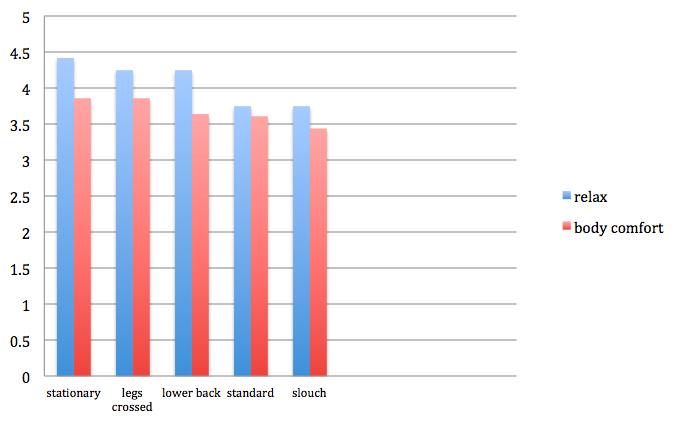
\includegraphics[width=0.5\textwidth]{figs/subjective}
\caption{The degrees of relax and body comfort to each posture}
\end{figure}

According to the subjective data alone, the slouch could be the top priority of our behavior regulation, as the lower degrees of comfort might indicate the higher risk to body injury. Based on this assumption, the order of the regulation followed the slouch should be lower-back-not-supported, leg-crossed, and stationary. However, the higher degrees of body comfort and relax could also indicate the measured posture is more frequently had by a subject. The assumption is supported by the fact that the standard posture, which should be the most appropriate and healthy one among the five, is only ranked at the fourth place with regard to the sense of relax and comfort of the participants. The participants might feel less comfortable when having a standard posture rather than a leg-crossed one, a lower-back-not-supported-one, or a stationary one because their bodies are not used to having such postures. The fact again proves the seriousness of the bad-posture issue.If the second assumption were true, the order of the posture regulation would be stationary, leg-crossed, lower-back-not-supported, and slouch. The analysis of the scenario study could help to determine the more reasonable assumption.

\subsection{Feedback Specification}

\subsubsection{Incentives}
Understanding the incentives for the users to improve their postures can be helpful in the feedback system design. The participants mentioned having better body shape, protecting eyes, becoming healthier, and feeling more comfortable as the main attracting points for them to improve their postures. 25 percent of them presented that seeing the research of an expert indicating the impact of bad postures would increase their willingness to improve their postures. Some participants from the 25 percent also mentioned that the knowledge from the research should be demonstrated using clear diagrams rather than lots of words. This might reflect the explanation path that the users' are convinced about the importance of having good postures could be a peripheral one. When taking a peripheral route, the user's' judgements would more likely be influenced by the source of information, humor, sexual hints, fear, and positive emotion (Petty and Cacioppo, 1986). Therefore, the system could deliver the feedback to a detected posture using the information from a credible source, or presenting the feedback in a way which makes people happy or exciting. Using the fear as a technique would not be considered because a positive user experience is emphasised.

The further investigation on the importance of different factors related to the posture improvement shows that the most critical reasons for posture improvement is owning a better body shape (37 percent), followed by becoming healthier (25 percent) and avoiding discomfort (25 percent), then is the last one, avoiding fatigue (13 percent). This could be explained by the assumption that the driving forces of having good postures (62 percent) might be stronger than the pushing force of avoiding bad postures (38 percent) on this issue. The assumption could be applied on the feedback system design such as using the techniques of positive reinforcements rather than the techniques of negative reinforcements. However, even though avoiding discomfort is classified as a pushing force, its high rating score still indicates the high concerns from the users and should not be ignored.

\begin{figure}[h]
\centering
  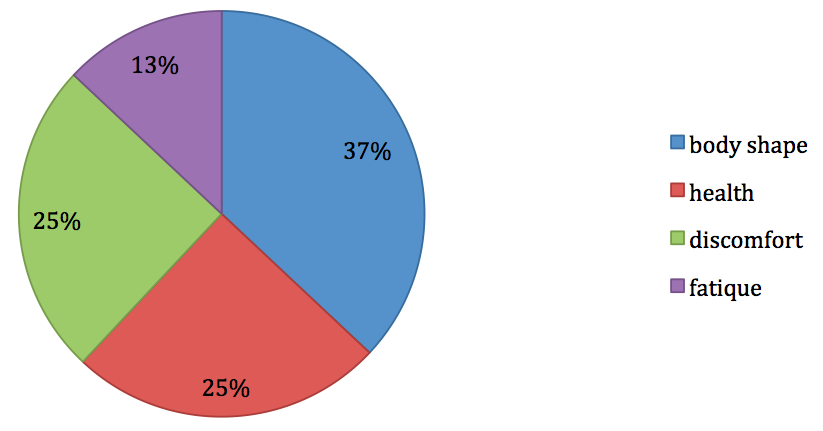
\includegraphics[width=0.5\textwidth]{figs/importance}
\caption{importance of incentives for having good postures}
\end{figure}

\subsubsection{Feedback methods}

There are five feedback methods to be compared with regard to the efficiency belief and the preference respectively. The candidates include simply presenting the current posture, presenting the current posture by a funny way, presenting the current posture by a cool or novel way, showing the impact of current posture, and providing compliments when the users are having good postures. The result of the investigation is illustrated in figure 4.6, as showing the impact of current postures is believed to be most effective, while receiving compliments for the good postures as well as knowing the impact of bad postures are most preferred. Providing compliments to good postures is highly ranked in both efficiency regard and preference regard, which means the feedback for improving the postures would not only help when bad postures show, but also when good postures does.

The result might also indicate that an informative feedback could be better recommended than a non-informative one, because showing the impact of current postures is apparently more informative than the others. The way to present the impact of current posture can be further discussed, however, the ranking of the methods to illustrate current posture could be analogous to the ways to demonstrate the impact of current postures. Namely, a cool/ novel way is slightly better than a cute/funny way, and the two are rated greatly higher than a simple way. Using a cool/novel way to show the impact of current posture is therefore identified as the most useful feedback methods based on the study.

\begin{figure}[h]
\centering
  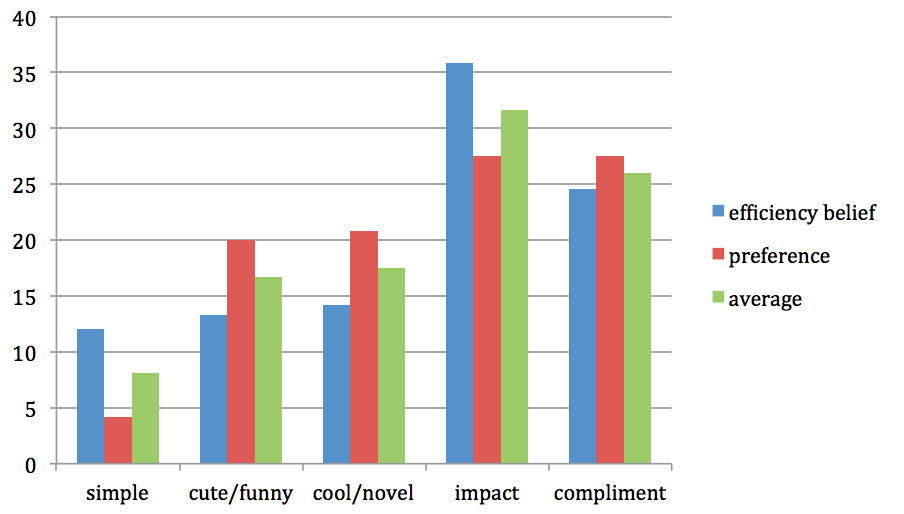
\includegraphics[width=0.5\textwidth]{figs/method}
\caption{Attitudes to feedback methods}
\end{figure}

\subsubsection{Feedback channels}
The posture feedback can be delivered within different perceptual channels among visual, audio, or touch. The audio channel is believed to be the most effective one, but its preference is just slightly higher than the visual channel, while the touch channel is significantly less identified with regard to both the efficiency belief and the preference. The difference of average scores between the audio and the visual channels should mainly contribute to the efficiency belief. However, such a strong efficiency belief for the audio channel could come from the property of an audio message, which is generally obtrusive. Due to this premise, the user experience design for applying audio feedback should be particularly considered.

\begin{figure}[h]
\centering
  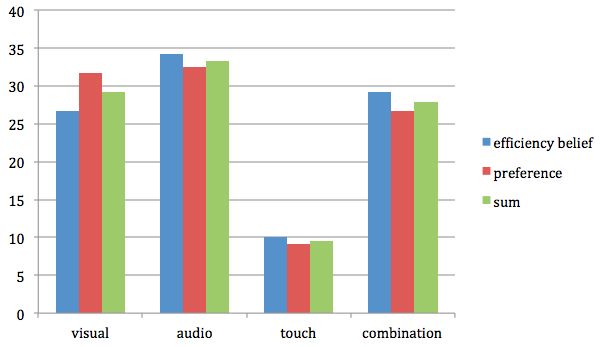
\includegraphics[width=0.5\textwidth]{figs/channels}
\caption{Attitudes to feedback channels}
\end{figure}

\begin{figure}[h]
\centering
  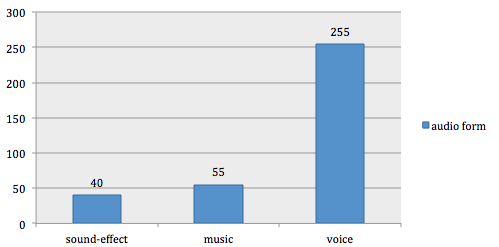
\includegraphics[width=0.5\textwidth]{figs/audioform}
\caption{Weighting for audio forms}
\end{figure}

The diagram of different audio forms shows the weighting value of the chosen audio form of each participant by their average ratings to efficiency belief and the preference for audio channel. Voice is rated as the most useful form, intensively higher than the other. Music is also graded over sound effect. This could also be contributed to the informative property as the analysis of feedback methods suggests.

The combination is generally defined as visual plus audio or all the three together. Interestingly, although the combination of using multiple channels is believed to be very effective, its preference is at least 10 percent lower than the visual and the audio. This might indicate the worry for the users to receive too complex information at once.

\subsubsection{Others}
The interview also investigated the actions that the participants have adopted for posture improvement. 66.67 percent of the participants said they never use any particular method to improve their posture. However, 37.5 percent of them said that they would remind themselves to avoid some postures, and 12.5 percent of them were given a kind of wearable equipment by their parents to avoid slouch in the childhood; All of them reported no effect for these. 8.33 percent of the participants indicated that they tried doing yoga for the purpose of improving postures, and it did enhance their posture awareness for half year, but the effect faded away when the participants stopped doing yoga. Another 8.33 percent of the participants said they could adjust the chair to make having a good posture more easily. Still 8.33 percent of the participants presented that they would ask themselves to decrease the usage the devices with visual displays and get away from the sofa, as the sofa is somewhere easily make people too relax and have bad postures. The other 8.33 percent of the participants claimed they would ask themselves to stand against a wall and this is helpful for them to remember the feeling of keeping the spine straight. The information of these methods could be provided if the suggestions for posture improvement are required by the feedback system.

\chapter{Feedback System}

\section{Overview}
Three functions chosen from the feedback model are implemented in this stage to construct the feedback system. The functions include \textit{Angel and Devil Clock}, \textit{Individual Head Tracking}, and \textit{Android Application}.

Angel and Devil Clock uses the projection system as the media to visualize how many users with either good and bad postures are currently detected in the environment. It also visualises the performance of the overall posture behaviour of all users in the environment, measured by the overall duration of their good posture and bad postures.

The second function is Individual Head Tracking. This function also uses the projection system as the media, and it will be triggered only it detects a user's bad posture. When the function is triggered, a spotlight will be projected onto the wall at the user's head position. If the bad posture had not been corrected in time, the spotlight would change into a blurry face, then a clear face, and eventually a body including a face and a skeleton. The joints affected by the current posture will be highlighted on the skeleton. The image will disappear immediately when the bad posture is corrected.

the bad posture reminding interval and good posture reinforcing interval

The android application is called \textit{ELF}, which is the abbreviation of \textit{Embedded Live-posture Feedback}. ELF demonstrates the feedback model when used cross-devices. The settings of the application can be personalised. The users can choose an avatar for their positive reinforcement, the reason to improve their posture behaviour, and the time interval to receive posture feedback. Once the application starts, it will serve in the background most of the time, and it will automatically jump out as a chat head when a good or bad posture of a user has remained over the user-defined interval. The user can click the chat head to open the messenger which shows the current posture type and its duration. The user can provide feedback by clicking one of the three emojis. The chat head then can be removed.

The system has two server-client connections. The computer connected to the Kinect serves as the first client, which passes the posture data to the first server. When the server receive the posture data, the compute would analyse the data and drive the projector to deliver appropriate Angel and Devil Clock and the Individual Head Tracking feedback. The same computer is also the second client that sends the posture analysis result to the server running on the mobile device.

\section{Angel and Devil Clock}

\subsection{objective}
The feedback aims to deliver the overall posture behaviour performance of all detected users in the environment. The rationale behind the design is hoping that social influence, such as social comparison, between users can impel them to improve their own posture.

\subsection{description}
All the graphics are hidden until any user in the environment is detected to have a good posture or bad posture. The angel figure will rise from the bottom at the first time when a user is detected as having a good posture. The same goes for the devil figure when a user is detected as having a bad posture. The two figures will be kept stationary until the system is closed. There will be some avatars on both the angel and devil’s arms. The number of avatars on the angel’s arm represents the number of the users who currently have good postures. On the other hand, the number of avatars on devil’s arm represents the number of the users currently having bad postures. The design of the avatars is a real-time reinforcement of good posture behaviours, because participants from the initial study wish that their good postures can be captured.

The angel is designed to give an impression that it is the better group, compared to the devil. It is shown through higher positioning of the angel compared to the devil, as well as happier avatars on the angel's arm compared to those those on the devil’s arm. According to the principle of social comparison, which states that people would reference others' behaviour and adjust their own behaviours based on their own judgements of what they observed~\cite{social_identity_comparison}, when some users are judged as belonging to the angel, other users would make extra effort to join the same party as the result of social comparison. If most users in the environment are judged as belonging to the angel’s party, there would be an effect of conformity on the remaining users. People tend to conform to what most people in the group do to avoid making themselves different from the norm~\cite{social_influence_complicance_conformity}.

The overall performance of all users' postures is visualized using tokens, where flowers represent good posture behaviours and boms represent bad posture behaviours. The performance score is calculated as the number of users with good postures multiply by the length of good postures minus the the number of users with bad postures multiply by the length of bad postures. If the performance score is positive, bombs will be removed and flowers will blossom. If the performance score is negative, flowers will gradually wither, and eventually when there are no blossomy flowers, bombs will appear one after another.

There is a good posture label and a bad posture label in the visualization. When a user initially joins either the angel or the devil, the corresponding label will appear for two seconds to indicate the user is represented by the newly added avatar on either the angel's or devil's arm. When a user changes from good to bad posture, or vice versa, the corresponding label will appear again. The labels are designed to remind the user's current posture behaviour, while reinforcing the association between the avatars and their posture.

\subsection{Design justification}
This feedback should give users a general understanding of their current posture behaviour. However, knowing their posture classification may induce the sense of fear or anxiety, for example, when users are classified into the devil's party. Therefore, the devil is drawn as a ridiculous, rather than terrifying, figure. In addition, the posture performance score is illustrated using flowers and bombs, as opposed to the original design of a clock. Not only do flowers and bombs depict the sense of positive and negative, respectively, feedback using static images compared to running clocks are less distracting to the users.

\section{Individual Head Tracking}
\subsection{Objective}
Individual Head Tracking occurs within the Angel and Devil Clock visualization. This feature emphasizes individual posture behaviours, whereas the Angel and Devil Clock focuses on both group posture patterns and the overall posture performance. This feedback has three levels, from subtle to obtrusive.

\subsection{Description}
When the system detects a user's bad posture, a spotlight will be projected onto the wall right in front of the user's head. The spotlight is a subtle feedback, as shown by its 30 percent transparency. The spotlight will also follow the user's head movement, until the user corrects their bad posture. The spatial position of the spotlight allows users in the environment to identify themselves, hence be aware of their bad postures.

Later, if the user has not corrected their posture after the spotlight is shown, a pair of eyes will be added to the spotlight, making the figure resemble a human face. According to Scheier \& Carver~\cite{self_focus}, the figure of eyes would facilitate the effect of self-focus, which makes the user more likely to be aware that they are currently exhibiting a bad posture.

Finally, when the user ignores the feedback again, a cartoonish skeleton will be displayed underneath the face. The body regions, or joints, that are affected by the bad posture will be highlighted. This feedback method is designed to provide users with information on the impact of bad postures on their body, which was rated the most useful by participants in the initial user study.

\subsection{Design justification}

The cartoonish skeleton is chosen over the default Kinect skeleton visualization in the SDK. There are three main reasons. Firstly, the Kinect has some uncertainties when it acquires joint positions, even when the user remains stationary. As a result, the user's projected skeleton joints would invariably move unpredictably along with the face. On the contrary, the cartoonish skeleton is a static image where all of the joints will move an equal amount of distance. Secondly, the posture reminder function is a supportive tool, hence the user should not pay too much attention on the details, for example, the joint positions. The user may spend more cognitive resources on the feedback visualization than necessary. Thirdly, users may find it embarrassing to share the skeleton joints with their companions. Moreover, this could threaten the privacy of self-space.

\section{ELF}
\subsection{Objective}
ELF provides posture feedback to users who are using their mobile devices and are likely to miss the information projected onto the wall. It also allows users to explore their current posture interactively.

\subsection{Description}
ELF is an android application. The homepage has two buttons - ``start'' and ``setting''. Users can click ``start'' to initiate the posture feedback service. Users can click ``settings'' to adjust the following settings: they can choose the preferred posture reminder interval, personal motivation for improving their posture, and the character which will praise their good posture.

The posture feedback service shows a small chat head of the elf saying ``I will serve you around.'' The chat head can be dragged to anywhere on the screen and hidden by dragging it to the bottom, just like the Facebook messenger chat head. If a bad posture has lasted for predefined, or the default, interval, the mobile device will vibrated. The chathead will reappear if it were hidden when a new feedback is received. The chat head image will have red edges if the user has bad posture or become an elf in Hawaii-vacation style if the user has good posture. If the user has a bad posture, the chat head will not be draggable until the user clicks on the chat head to open the messenger.

The messenger has three sections. The elf will display the current feedback with an animation, a short description, the duration of the posture, and a timestamp. The user can respond to the posture by clicking one of the three emojis to show their current feeling. The emojis include a determined face, a calm face, and an annoyed face. The system will display a text for each emoji the user choses. For example, if the calm face were chosen, the system would show ``Ok! I understand''. The emojis are an application of cognitive dissonance. The system displays a message that is far more positive than the actual emoji, even for the annoyed face. Therefore, the user would tend to adjust their actual feelings to keep it consistent with the displayed message. Then, the elf will reply to the said message, while reinforcing the same idea with cognitive dissonance.

When the user has a good posture, the system will display the character selected by the user in the setting panel saying ``Nice Posture!'', instead of an animation. According to the transportation theory proposed by Green (2004), when people like one character, they tend to identify with what the character says and does. The statement ``Nice Posture'' could be an effective reinforcement of the user's good posture behaviour.

\subsection{Design justification}
The elf in the home page wears a suit, which gives a sense of professionalism. According to the elaboration likelihood model proposed by Petty and Cacioppo~\cite{elaboration_modeL_persuasion}, the user would more likely be persuaded by information provided by an expert. The user study also shows that users tend to take the cognitive peripheral route when deciding their posture, that is, they do not think too much before doing it. The elf is displayed as a credible source which the users can use it to guide their posture behaviour. In addition, Petty and Cacioppo~\cite{elaboration_modeL_persuasion} also suggest that keeping people in a good mood would facilitate persuasion procedure when people take a peripheral route. This gives rise to the relaxing style of the graphics in the current application.

\section{Implementation}
These feedback contain many graphical materials. All of the graphics are designed and created originally, except the pictures of the characters used to complement good postures and the cartoonish skeleton.

The Angel and Devil Clock and the Individual Head Tracking are implemented using \Csharp{} in Visual Studio. The project is based on the Microsoft RoomaliveToolkit~\cite{roomalive_toolkit}, as it supports projection mapping for the system. Using the Roomalive Toolkit also enables other functions in the feedback model having the 3-dimension effect to be integrated in to current system. The drawing of the graphics feedback to be projected is conducted using the Windows Forms class. The computer connected to the projector is the server that receives the data passed from the computer connected to the Kinect, and it would use the classification model to render the appropriate feedback for current posture and drive the projector to deliver it. In the meanwhile, the computer would pass the data related to current posture to the android device to activate the ELF.

The ELF is implemented using Java in Android Studio. It includes four activities and six layouts. The mobile device is the server, which receive the data passed from the client. The data is used to determine the content of the feedback. The server and client are from Kinect2Kit\cite{kinect2kit}. The two server-client pairs integrate the functions of the posture detection, posture classification, and the three functions provided by the two devices for the system.

\chapter{Evaluation}

\section{Objective}
The study aimed to assess the usability of the current system by analysing the objective data of target posture occurrence rate in the scenario study, and the subjective data of the participants’ perspective to the system on 8 dimensions for the usability.

\section{Method}
The study included two sections. In the first section, the participants were randomly assigned into either watching TV group or using mobile device group. A Kinect would be placed in the front of where the participants sit to record the position of 25 joints in the body and a DV would videotape from the side. The participants were be asked to relax and behave like they usually did when engaging in the tested activity. Both scenarios would last for 15 minutes. Participants in the watching-TV group would watch a talk show, while the participants in the using mobile device group would be given an android phone, with the ELF installed, to use within the time. As watching TV is an activity that enables many people to engage in at the same time, the study had 2 pairs of participants to attend the scenario study together, and three participants to attend the scenario individually. On the other hand, four participants were assigned to attend the using mobile device scenario individually since it is an activity usually conducted by oneself. In summary, there would be 4 participants attending the scenario of using mobile device individually, 3 participants attending the scenario of watching TV individually, and 4 attending the scenario of watching TV individually.

The second section was an interview to investigate the perspectives of the participants to current system. Some questions were chosen from the
\textit{System Usability Scale}~\cite{sus}, as the scale was tested to have great reliability in the evaluation of a variety of applications. The other questions were generated originally to test six heuristics related to the use of current system, namely consistency and standardization, flexibility, efficiency, aesthetic and minimalist design, match between the system and the real world, and the consumption of the working memory, among the 10 usability heuristics proposed by Nielson~\cite{nielson_heuristics}. Nielson's heuristics were referenced here as they could be regarded as the principles of usability. In addition to the 6 heuristics, there were also some questions investigating the experience of receiving the feedback from each feedback functions, and a question to ask the frequency that the participants would like to use the system when they were at home. The questions were grouped to explore the 8 dimensions of usability for the system respectively.

\section{Participant}
11 university students aged between 20 and 30, body height between 155 and 173 cm (average = 165.1), with no significant musculoskeletal disorder history.

\section{Material}
\subsection{Experimental apparatus and resources}
The following materials were used to measure the posture, record the procedure, construct the system, and facilitate the interview.

\begin{itemize}
\item A Microsoft Kinect
\item A digital video
\item A projector
\item A TV display
\item A speaker
\item An android phone
\item Two computers
\item Interview statement sheet (See Appendix~\ref{appendix:interview_instructions})
\end{itemize}

\subsection{Documents for ethical concerns}
The ethical considerations of the study were approved by The University Teaching and Research Ethics Committee. The approval letter for the study could be seen in Appendix H. The following sheets were given to the participants to protect their right and ensure they understood the study.

\begin{itemize}
\item Participant Information Sheet (See Appendix~\ref{appendix:information_sheet})
\item Participant Consent Sheet (See Appendix~\ref{appendix:consent_form})
\item Participant Debriefing Form (See Appendix~\ref{appendix:debrief_form}) 
\end{itemize}

\section{Procedure}
The researcher would introduce the system as well as the objective of the study to the participant in the beginning, and ask the participant to read and sign on the consent sheet and the information sheet. The participant would be assigned into a scenario, and the scenario would begin when the participant reported he was well prepared and relax. The scenario would last for 15 minutes, with a DV videotaping from the side. After the scenario, an interview would be conducted to investigate the participant’s perspective on the usability of the system. The contents of the interview can be seen in appendix F. A briefing procedure following would enable the researcher to again explain the purpose of the study, and encourage any opinion which aroused during the study to be reported.

\section{Result and Analysis}
\subsection{Scenario Study}
In the first scenario, the participants would be asked to relax themselves and use the provided mobile device to do whatever they liked. They would receive the feedback for their postures from the android application on the mobile display and the projection system on the front wall. The participants in the scenario were detected as crossing their legs on average for 4 percent (standard deviation = 2.73) of the time, slouching for 15.3 percent (standard deviation = 6.67) of the time, and having a low viewing height for 28 percent (standard deviation = 47) of the time. The standard deviation for having a low viewing height posture was high because one participant had the posture for 98.5 of the time while the others had the posture for approximately 5 percent of the time only. Figure~\ref{fig:scenario_mobile} shows the comparisons of the target posture occurrence rate before and after the current system was applied. The occurrence rate of crossing legs decreased by 90 percent, while slouch and low viewing height also decreased by 38.9 and 35.6 percent respectively.

\begin{figure}[h]
\centering
  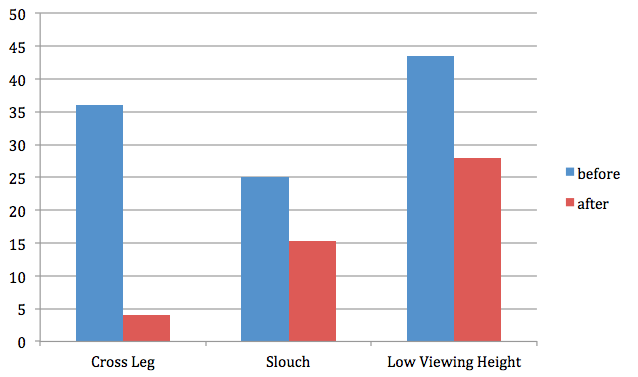
\includegraphics[width=0.5\textwidth]{figs/scenario1}
\caption{Posture occurrence rate comparison before and after the use of system in mobile device scenario}
\label{fig:scenario_mobile}
\end{figure}

In the second scenario, the participants would watch a talk show on TV and receive the feedback for their postures from the projection system on the front wall. The participants were either doing the activity by themselves or being paired with one friend. In the former condition, the participants were detected as crossing their legs on average for 12.84 percent (standard deviation = 17.1) of the time and slouching for 30.5 percent (standard deviation = 12.23) of the time. In the later condition, the participants were detected as crossing their legs for 24.5 percent (standard deviation = 4.91) of the time and slouching for 54.38 percent (standard deviation = 11.12 percent) of the time. Figure~\ref{fig:scenario_tv} shows the comparisons of the target posture posture occurrence rate before and after the current system was applied. For the participants watching TV individually, the occurrence rate of cross-leg posture decreased by 63 percent, and slouch posture decreased by 59.2. For those watching TV with another participant, the occurrence rate of cross-leg posture decreased by 29.4 percent and slouch posture decreased by 27.3 percent on average. 

\begin{figure}[h]
\centering
  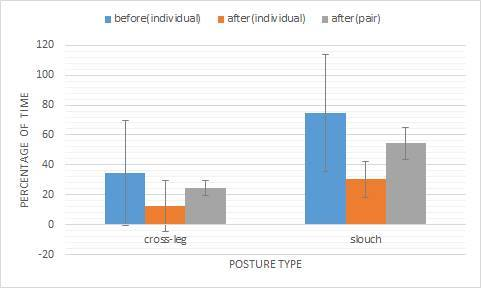
\includegraphics[width=0.5\textwidth]{figs/scenario2}
\caption{Posture occurrence rate comparison before and after the use of system in TV scenario}
\label{fig:scenario_tv}
\end{figure}

The deviation of the posture behaviour occurrence rate was caused by the small amount of participants in the study and the diversity of posture behaviour between people. The deviation of the posture behaviour in the evaluation study, however, was less than the deviation of the posture behaviour measured in the prior user study. This might also indicate that the system had some effect on the posture improvement therefore the diversity of posture behaviour pattern between the participants decreased. The procedure for the participants to change their posture behaviour pattern could be explained using the Yale attitude model. According to the Yale model, the participants should first \textit{pay attention} on the feedback, then \textit{comprehend} the content, and \textit{accept or agree} with the information. The information should be also \textit{retained} in their mind until they \textit{take action}~\cite{communication_persuasion}.

To sum up, the system improved all target posture in every scenario basically, which meant the system achieved its aim possibly using the Yale attitude model. The system had the best effect on improving cross-legs posture (90 percent in using mobile scenario and 63 percent in watching TV individually scenario) among all target bad postures. Also, the system had better effect on improving target postures when there was only one user in the environment than two users. It might because that the interaction among the users could cost their cognitive resource and reduce the possibility for the feedback in Yale model to go from one stage to another, such as the information of the feedback might stick in the stage of acceptance without continuing and enter the stage of retaining. The candidate solution for the problem would be discussed in next chapter.

\subsection{Interview}
The interview focused on eight dimensions of the system. Each dimension was assessed by the participants’ rating for one to five statements. The list of statements can be seen in Appendix F. The index of the dimension and its corresponding statements are presented in Table 6.1. The scores of the reverse statements would be calculated backwards, and the average and standard deviation scores of each dimension would be examined. The result is presented in Figure~\ref{fig:usability_ratings}.

\begin{table}[ht]
\centering
\begin{tabular}{l c c}
Dimension&Statment Amount&Statement Nimber\\
\hline
Consistency and standardisation&2&1,2\\
Recognition rather than recall&1&4\\
Match between the system and real world&1&3\\ 
Flexibility&1&8\\
Efficiency&5&5,6,7,9,10\\ 
Aesthetic and minimalist design&2&11,12 \\
User experience&3&13,14,15\\
Frequency of use&1&16\\
[1ex]
\hline
\end{tabular}
\label{table:nonlin}
\caption{Index of Usability Dimensions and Corresponding Statements}
\end{table}

\begin{figure}[h]
\centering
  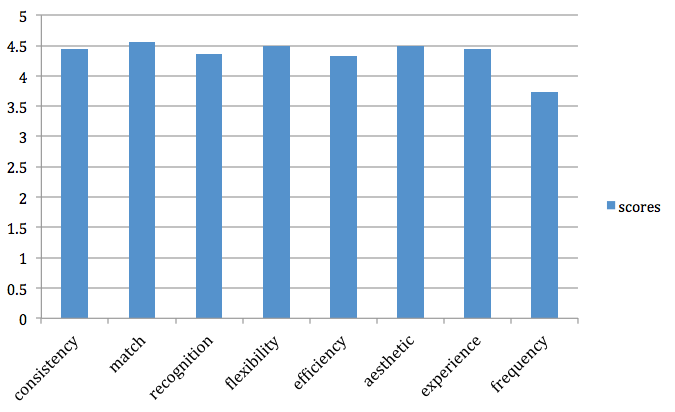
\includegraphics[width=0.5\textwidth]{figs/dimension}
\caption{Average ratings for each usability dimension on 5-point scale}
\label{fig:usability_ratings}
\end{figure}

The ratings between the participants were consistent in most statements. The average standard deviation of ratings for one statement was not higher than 0.7 in every dimension excluding the frequency of use. This is because some of the participants reported that they might not always want to improve their postures; sometimes they just wanted to relax in a comfortable posture and pay no consideration about whether it is a healthy posture or not. With the comparative high deviation, the average rating for the predicted frequency of use was also the lowest one among the all. The average 3.73 indicates the frequency for the participants to user the system would locate between sometimes and often. The other dimensions, on the other hand, were given high identification in general. The evaluation of the feedback system could also verify the posture model by including the statement of \textit{the system could catch my posture sensitively} and \textit{the system could categorise my posture correctly} in the efficiency dimension. The two statements were rated for an average 4.09 and 4.0 respectively.

The open-ended questions following investigated the perspectives of the participants to the three feedback functions respectively. The analysis was made by the interpretation of notes taken in the procedure of the interview.

\begin{enumerate}
\item Angel and Devil Clock feedback \hfill \\
The participants reported that they felt the design of the system was novel and special, and wanted to be classified into the party of angel. However, they mentioned that the system could catch their attention due to its attractive design, but also could distract their attention sometimes particularly when the label flashes when a user was firstly classified as having a good or bad posture. Also, the flowers and the bomb were respectively used as the tokens of the accumulated good posture lasting time and bad posture lasting time, but the flowers would wither due to the increase of accumulated bad posture lasting time, while the bombs would just disappear subsequently when the good posture lasting time increased. Namely, the tokens for the good posture behaviour, flower, has two types, but the tokens for the bad posture behaviour, bomb, only has one. The imbalance might confuse the users.
\item Individual Head Tracking feedback \hfill \\
Some participants felt a little bit creepy when the eyes in the face firstly show. After that, they felt the effect of the skeleton was novel and useful when the constrained joints being highlighted. They reported that they would perceive the skeleton on the wall as the reflection of the negative part of themselves, and try to wipe it out. For the downside of the design, a participant mentioned that if the user were sitting at one side of the sofa and watching a TV located in the front of the other side, the feedback could be easily ignored because the image of the spotlight would be projected on to the position where right in front of the user as the feedback for a bad posture. As there would always exist the problem of blind point for a visual feedback, the integration of the Individual Head Tracking and some audio effect could be effective. The comparison of using the cartoon-style skeleton and the user’s real skeleton image (the picture of Kinect Body Basics would be introduced) was also investigated. About 2/3 of the participants preferred the cartoon-style skeleton, because it would be less scary, and would not cost that much attention to look at compared to the amount that would be cost in their imagination. The other 1/3 said using the skeleton of the user himself would be cooler and further increase the user’s sense of involvement on the promoted issue.
\item ELF \hfill \\
Generally the participants were satisfied with the application, as it could serve in the background, easily be modified, and interact with the user by providing personalized encouragement to the user’s selected emoji. One participant suggested the system to include more emojis and increase the possible interactive methods between the user and the system, which could be a great progress for the future work. However, the analysis of the data show a drawback of using the mobile device to provide the posture feedback: the participant who behaved as most being fascinated by the application was examined as having a low viewing height posture for 98.5 percent of the time when the participant was immersed in the using mobile device activity and tried hard to explore the different functions provided by the application. Using the feedback delivered by a mobile device, which would possibly be viewed with a low viewing height posture as well, to improve the low viewing height posture could be really challenging. Other feedback form, such as an audio effect, could be integrated with the functions provided by ELF, so that the user could no longer tend to check a feedback for a low viewing height posture with a low viewing height posture. However, other media could still have better effect and be more appropriate for the improvement of low viewing height posture.
\end{enumerate}

The analysis in this chapter mainly focused on the findings from the evaluation study. More considerations and limitations about the system will be discussed in the next chapter.

\chapter{Conclusion and Future Work}

\section{Current Work}
In this research, the researcher built a posture feedback system with three feedback methods and decreased the occurrence rate of every target bad posture in every scenario.

The system defined its target bad postures for the system based on a trade-off between the combinations of health posture principles and a predictable comfortable and relaxing user experience, generated from the NHS guideline~\cite{nhs_sit_correctly}, Torres~\cite{best_viewing_distance_tv}, and Hargrove~\cite{bad_posture_back_pain} (See Table~\ref{tab:posture_descriptions}). A feedback model listing 33 candidate feedback methods (see Figure~\ref{fig:feedback_model_2}) is built to discuss the appropriate response to the detected posture.One of the main features of the feedback model is that it contains multiple output devices, which enables the researcher to broaden the diversity of candidate feedback methods. The feedback model also groups the candidate feedback methods by three intervention extends, which are subtle, subtle to obtrusive, and obtrusive respectively. The methods with less intervention extend would be delivered earlier to minimise the interferences to the user's’ current activities.

A posture classification model developed in the user study is responsible for the real-time posture type judgements.The model has high accuracy rate on classifying detected postures according to the result of validation and evaluation. Once a classification is made, an appropriate feedback would be delivered accordingly. The design of the feedback system are mainly based on the findings from the user study and the literature review. There are three feedback implemented in the system: Angel and Devil Clock, Individual Head Tracking, and the android application ELF. The functions are integrated using two pairs of client and server. The functions support the reinforcement for good postures, the illustration for overall posture behaviour performance, the active explore for the current posture, and the demonstration for the impact of current posture. The system also provides the cross-device feedback, using the projector and the mobile device in the same time to decrease the possibility for the user to miss the information.

The evaluation of the system presents the improvement of the bad posture occurrence rate on every scenario, and also shows an average rating 4.4 from the 5-point Likert scale for the eight dimensions (see table) of the system.

\section{Limitation}
There are four main limitations for the system. Firstly, the effect of the feedback for the stationary posture and the short viewing distance are not tested in the study. It is because the nature of a stationary posture, which is defined as all joints in a body region (with +-0.04 cm tolerance for the measured value) being kept in the same positions for 15 minutes in this research. The observation duration for the scenario is also 15 minutes only, as the scenario observation is just a part of the evaluation; if the overall length for the evaluation lasted too long, there could be a problem for the participant recruitment. On the other hand, if the definition of the stationary were modified for the purpose of testing the effect of the feedback for it, a user who keeps a good posture for a reasonable time would receive a bad posture feedback saying their good posture is too stationary, which would be disruptive and influence the trust for the user to the system. Therefore, the evaluation for the effect of feedback for the stationary posture is not available currently. A natural short viewing distance posture behaviour is also unlikely to be observed due to the limit of the lab setting.

The second is about the limitation of the Kinect, which is used as the only tool to gather the posture data. If a user keeps stationary for a while, the Kinect might regard the user as the background until the user moves again. This circumstance did not show during the tests, but it is likely to happen when the system is applied into real life. An additional condition could be added into the judgment system, such as, if the head position of any user were not cross the border of the Kinect’s observation scope before the user disappears, the user should be regarded as staying in the position where they are lastly detected, and the feedback for a stationary posture should be delivered.

The third is the predefined setting for the environment due to the use of a projector. Most projectors can only project clear image in a dark environment due to its principle of operation. Currently the projectors that can perform well in the bright environment are usually expensive and mainly for research use. However, the breakthrough of the technique and the popularization of the powerful projector are predictable.

The fourth limitation could be the biggest challenge for the system to be applied in real life, which is the reliability of current posture classification model. The current model was built using the data from only 10 participants and validated with the data of only 2 participants, with body height ranged between 156 and 172 cm. The amount of the participants is not representative to all potential users. A model built and validated with the data from more participants that cover all body height ranges would be more reliable and effective, and the demographical issues could also be considered into the procedure of the model construction. Building different models for different groups of the users could be a possible solution to achieve a good reliability and validity for the model. Also, the Kinect sensor. should be placed on the ceiling to prevent the blocking in real life application.

In addition, the user study for the watching TV scenario only measured the posture behaviour pattern of the participants who engaged in the activity alone, but the posture behaviour pattern of the participants engaged in this activity with a companion were also assessed in the evaluation. The comparison between the two scenarios could not really reflect the effect of the system for improving the posture behaviours of two users at the same time, as the baseline data is not of the same condition. The design of the experiment could be improved in the future research and a more reliable result could be found. Further, the scenarios of watching TV are not limited in individually or two persons, the scenarios for more people watching TV could be studied in the future research.

\section{Discussion}
\subsection{Social influence}
The system achieve its predicted effect in general, however, the improvement for the posture behaviour when two users watching TV together is not as good as the other scenarios, if the bias for using the data of watching TV with only one participant as the baseline were temporarily put aside. The expected power of social influence, such as social comparison and conformity, seemed not work significantly. This might because that the users did not notice the other people’s posture classification or care this enough, as this issue might not that matter to them to spend the cognitive resource on.

There would be two possible ways to enhance the effect of the social influence. The first is to increase the user's’ emphasis on the posture behaviour by providing more prior instructions about the importance of having good posture. If the user emphasises the posture behaviour more, they would be more likely to observe what posture the others have and what’s the classification for it. The effect of social comparison is therefore more likely to work. The other method is to use the power of the social cohesion, which is defined as the power that make people from the same society to cooperate with each other for the good of the society~\cite{elaboration_modeL_persuasion}. As the system is used for home setting, the users from a same environment would usually live together and be close to each other, which could be regarded as a team; if there is an online platform built for the performance of the team’s overall posture behaviour to be uploaded, and some appropriate and appealing reward could be given for the teams with good performance, having good posture behaviour could become a common goal of the users from a same team. The effect of social cohesion could happen.

\subsection{System performance}
The result from the evaluation could be an underestimate to the system's actual performance, since most of the participants presented they felt the effect of the system is novel and therefore intended to have many different postures to explore the system. The fact again backs the efficiency for the system in short term. On the other hand, the long-term performance for the system did not be evaluated. If the users get used to the stimuli provided by the system, the desensitization of the user to the system is possible to happen. The users would be more and more easy to ignore the feedback for their posture, especially for who hold a passive attitude for the posture improvement.

There could be two possible solutions for the desensitization issue. The first one is to modify and update the system from time to time. For example, change the pattern of the angel or the devil’s clothes, or change the tokens for good posture performance with different species of the flowers. However, if the change is not significant and interesting enough, the desensitization would still happen. The only way to ensure the system's long-term performance is to enhance the user’s emphasis on their posture behaviour. If the user put enough emphasis on the posture behaviour, they could become an active user and increase the priority of their limited cognitive resource use on the information provided by the system. Some diagrams or pictures, which indicates the importance of having good posture and are relevant to the issues that the user cares, can be provided every time the user starts the system to influence the attitude for the importance of good posture. For example, the diagram showing the difference of average thickness of legs between people who often have a cross-legs posture and people who don’t could be persuasive for the users who care their body shape very much.

\section{Contribution}
There are three main contributions of the research. The first one is the construction of an effective posture classification model. The model is linear and enables the classification to be made in real-time. Also, the performance of the model is good according to the participants’ rating (sensitivity = 4.1 and correctness = 4.0 on a Likert 5-point scale). Using the posture data from more participants in a future user study to modify the parameters in the formulas of current model could further increase its reliability.

Secondly, the feedback model generated in chapter 3 provides abundant candidate feedback methods. There are 34 feedback methods in the model and can be categorised by targeting posture, output device, and intervention extend. Future researchers who aim at designing the feedback to improve posture or regulate a specific can reference the model and modify the methods within to apply to their work.

The third and the most important contribution is the development of a new feedback system for posture behaviour. The system is very different from the past works sharing the same objective, such as a wearable device for slouch feedback~\cite{wearable_spinal_posture} and the ergonomic-based sitting apparatus for maintaining a good posture~\cite{monitor_support_apparatus}. It provides cross-device visual feedback and is able to recognise different type of bad postures. More importantly, the system emphases the user experience very much. The feedback it delivers would have only subtle intervention extend, which gradually increase along the duration of the detected bad posture. Also, the contents of the feedback are carefully chosen and what might cause anxiety or fear to the users is avoided.

\section{Future Work}
\subsection{Posture classification model}
A more reliable model is needed for the posture classification. It should be built using the data of participants that cover all body height ranges, and the demographical issues could also be considered. It might require multiple models that suit different groups of the users to ensure an accurate and reliable classification quality. In addition, currently the Kinect sensor is placed on the table in front of the users; however, the vision of the sensor would be occluded by other stuffs in the real life setting. The solution would be to install the Kinect sensor at the ceiling and observe the users from upside down. The parameters for current posture classification formulas should also be modified accordingly.

\subsection{New functions}
The improvement of current system includes five dimensions. The first dimension is to integrate some audio feedback into the feedback system. For example, when current intervention extends of feedback is obtrusive, which means the detected bad posture has already kept for a while, some sound effect can be added to further remind the user about their posture. This would be particularly useful when a feedback for a low viewing height posture is needed in a using mobile device scenario. The action for the user who get used to have a low viewing height posture when using the mobile device to receive a visual feedback for the posture on a mobile device, often make the user to repeat the posture. Therefore, an additional audio feedback could be helpful.

The second dimension is to build an online platform to enable the performance for the posture behaviour of each user team automatically uploaded. The function could hopefully trigger the social influence of social cohesion and conformity for the users on the task of posture improvement. The third dimension is to show the diagram or the picture, which is easily understandable and relevant to the considerations of having good posture for the user, every time when the user start or close the system. It is for improving the attitude of emphasis towards the importance of posture, and the emphasis of having good posture to some extend is a premise for the system to have a long-term effect

The fourth dimensions is to increase the amount of the stages for the Individual Head Tracking to provide from the spot to the skeleton. The spot could change from very transparent to not transparent, and the eyes could appear from very vague to clear. This would make the feedback at the beginning more subtle and reduce the interference to the users.

The fifth dimension is to make a user interface to provide the user with some flexibility to customise the system within some extends. The user could be allowed to set the size and the position of the angel and devil figure, as well as the flower and bomb. They could also adjust the size and colour of the avatar, which are their representatives. The function could not only enlarge the flexibility of the system, but also increase the degree of the favour the users hold to the system.

The implementation for the functions of the four dimension with a refined posture classification model can be expected to enhance the usability of the system especially on the efficiency, flexibility, and user experience aspects, and also increase the effect for the user's' posture improvement. Some new feedback methods could also be added into the system after the evaluation procedure.


%now enable appendix numbering format and include any appendices
\appendix
\chapter{Output Device List}
\label{appendix:output_devices_list}

According to Computer Help~\cite{output_device}, general output devices include:

\begin{itemize}
  \item 3D Printer
  \item Braille embosser
  \item Braille reader
  \item Flat panel
  \item GPS
  \item Headphones
  \item Computer Output Microfilm (COM)
  \item Monitor
  \item Plotter
  \item Printer (Dot matrix printer, Inkjet printer, and Laser printer)
  \item Projector
  \item Sound card
  \item Speakers
  \item Speech-generating device (SGD)
  \item TV
  \item Video card
\end{itemize}

\chapter{Instructions for User Study}
\label{appendix:instructions}

\section{Opening}
Hi, thank you for coming to participate my experiment. The aim of my dissertation is to develop a system that can detect people’s posture and provide real time feedback. Your participation would be helpful for me to model some postures and find the general behavior pattern in some scenarios. Please read the information sheet and sign on the consent sheet. If you have any question, you are welcome to ask anytime.

\section{Section 1}
In the first section, we are going to measure some postures. Please relax and sit on the chair with my appointed posture. If you have any question about the appointed posture don’t hesitate to ask. You can do any activity you like such as using your smart phone or watching TV. First, please sit properly in your most comfortable and usual way.

(After three minutes) This is the first part of this section. Now I would like to ask you some question about this your experience on the posture and your answer should range between 1 to 5. 5 is very positive, and 1 is very negative:

\begin{enumerate}
  \item To what extend did you relax?
  \item How's the similarity between your posture in current condition and in your daily life?
  \item Please also feel your body. How’s the current comfort to your neck?
  \item How’s the current comfort to your shoulder?
  \item How’s the current comfort to your spine?
\end{enumerate}

(The procedure would be repeated for each posture according to the order of the assigned group for each participant)

\section{Section 2}
The second section is a scenario study. Your task is to sit on the sofa and use your own mobile device/ watch the TV. (If the participant asked anything about postures, answer ``just make yourself at home.'')

(After 15 minutes) Time's up. To what extend did you relax when you were doing the activity? How similar there is between your current posture and your usual posture in this scenario? 

\section{Section 3}
The section three is a brief interview.I would like to understand more about your posture pattern and the way that might help you to improve it.\\

\begin{enumerate}
  \item First, do you have any musculoskeletal disorder history? If any, do you mind to specify it?
  \item Do you have any musculoskeletal discomfort in the past three months and why do you think they come?
  \item To what extend do you think your posture is appropriate and healthy? 1-5
  \item How often are you aware that you are having bad postures? In what timing are you usually aware that you are having bad posture?
  \item What effort did you make to correct bad postures? (Method, duration, result)
  \item What can motivate you to have better postures?
  \item Can you distribute the 100 tokens to different benefits of having good postures according to their importance to you?
  \item Can you distribute the 100 tokens to different feedback methods according to the efficiency you believe it can have for you when you are at home?
  \item Can you distribute the 100 tokens using the same table according to the willingness for you to install such a system at home?
  \item Can you distribute the 100 tokens to different perceptual channels, which can be used to receive the feedback of posture at home, according to the efficiency you believe it can have for you?
  \item Can you distribute the 100 tokens to different perceptual channels, which can be used to receive the feedback of posture at home, according to your preference for receiving such kind of message in the form?
\end{enumerate}

\section{Wrapping up}
The experiment is finished.If you feel any physical uncomfortable,a consulting service is available by calling 111. If you are interested in the result of the research or the analysis of your personal data, please leave your email address and I am very happy to send you a copy of it after it is done. Thank you for your participation. Good bye!

\chapter{Consent Sheet for User Study}
\label{appendix:consent_form}

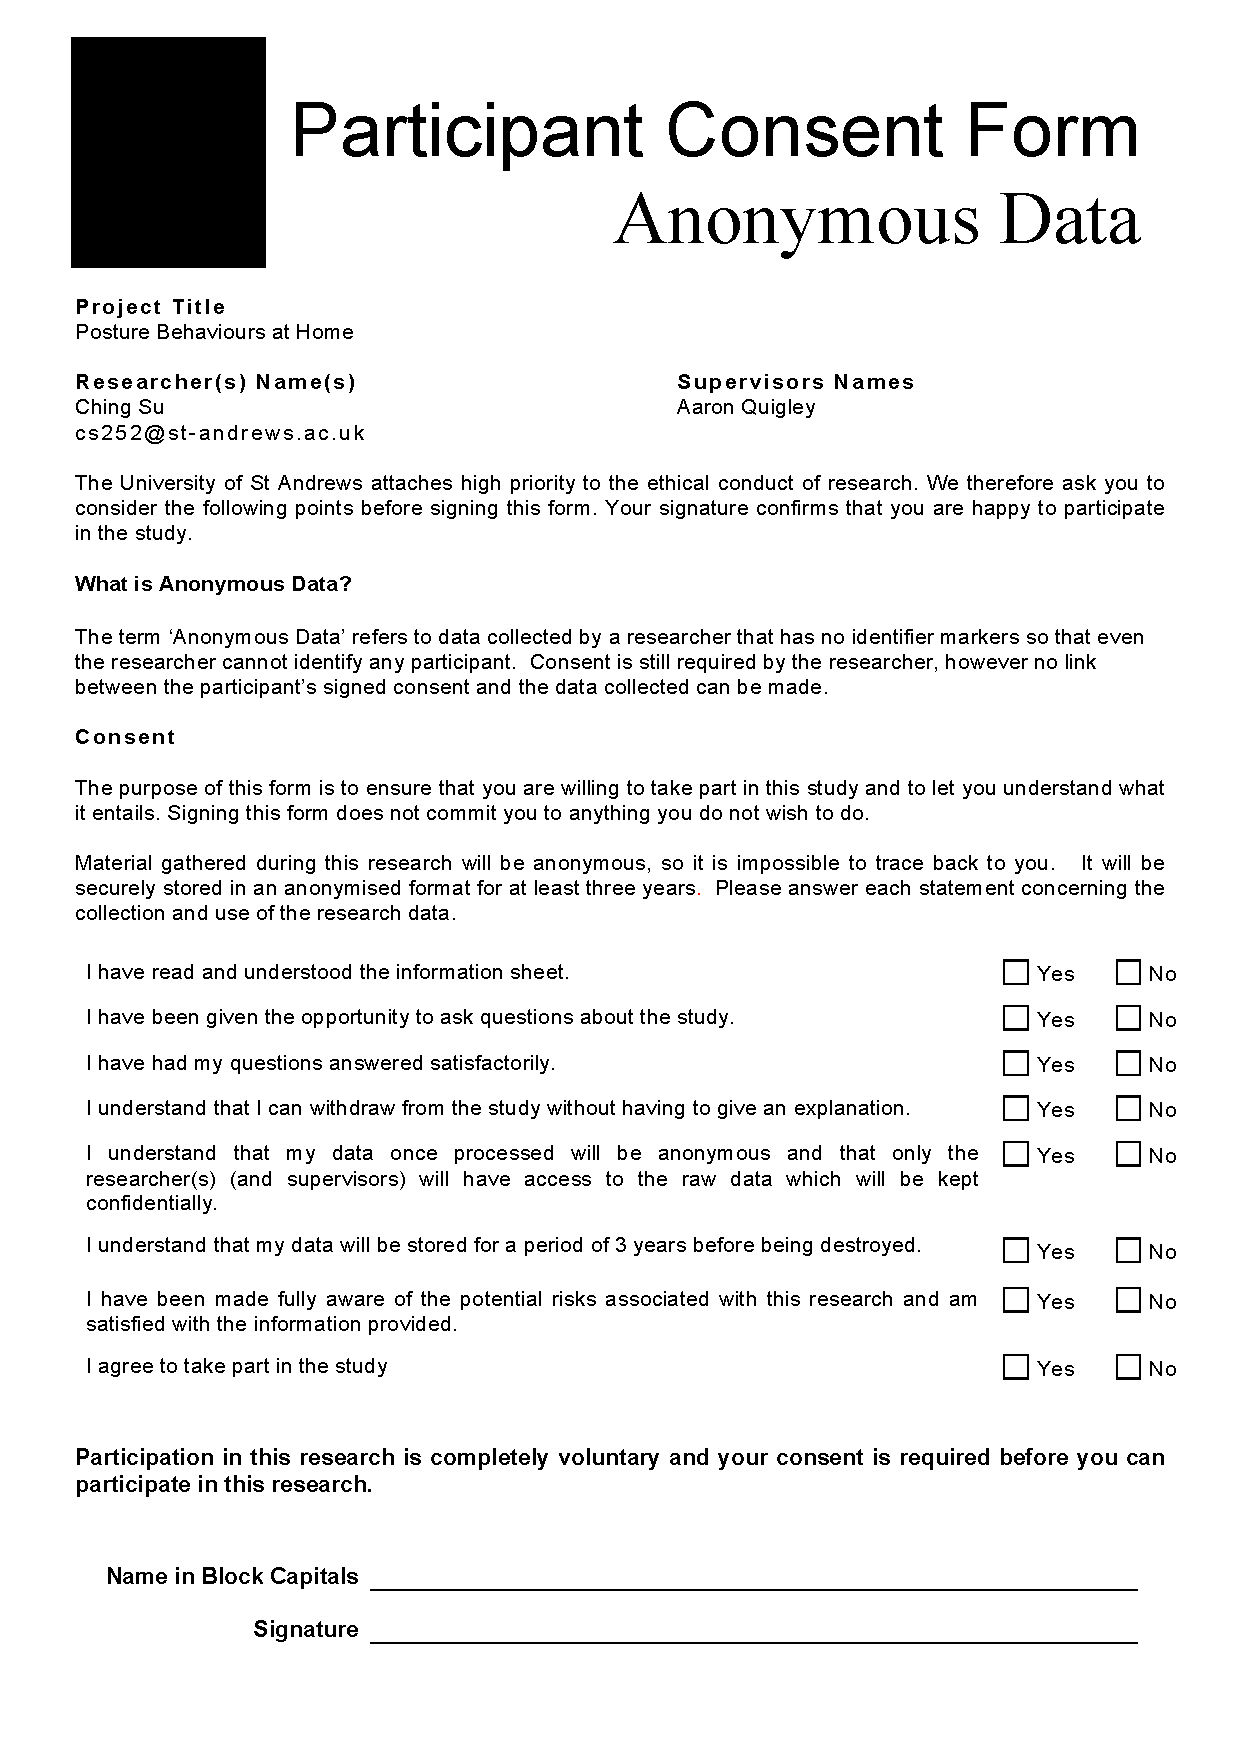
\includepdf[pages={-}]{ethics/consent.pdf}

\chapter{Information Sheet}
\label{appendix:information_sheet}

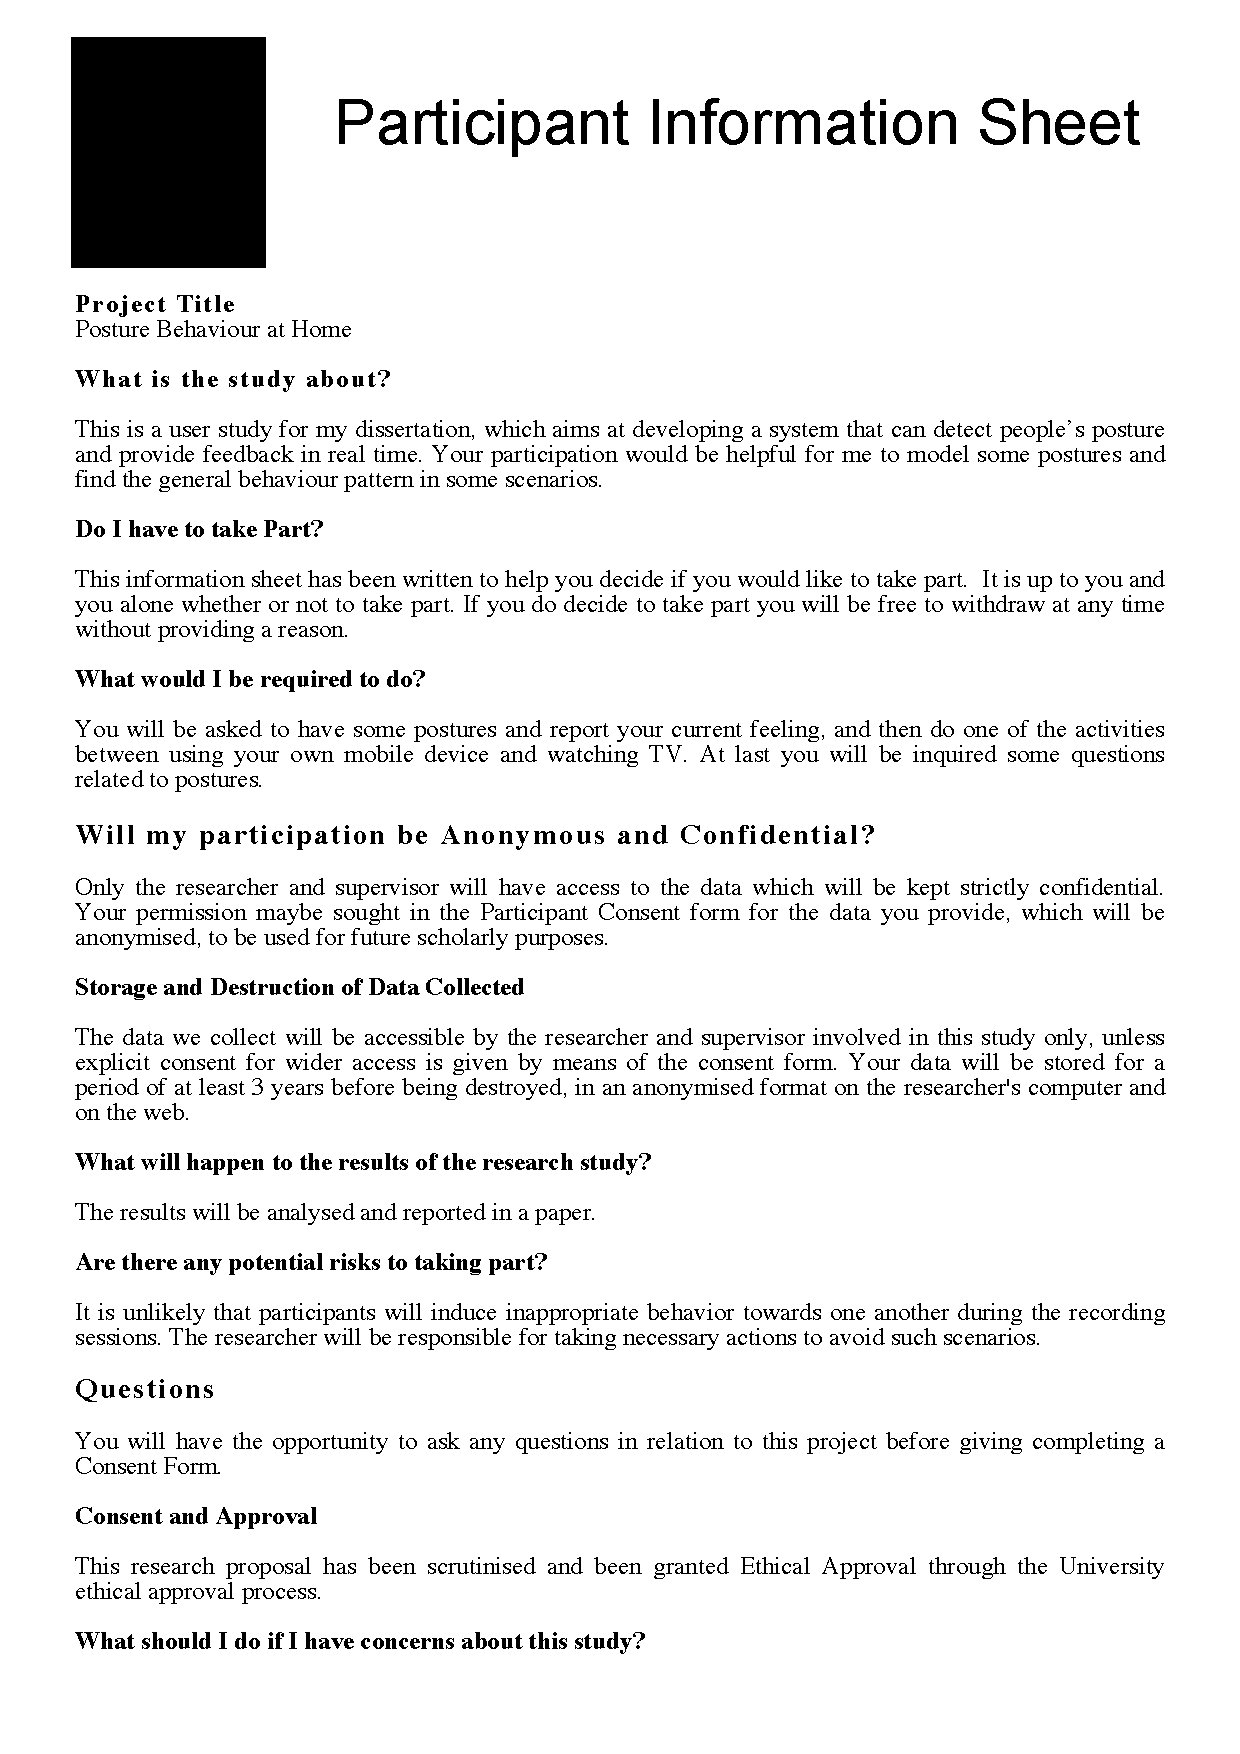
\includepdf[pages={-}]{ethics/information.pdf}

\chapter{Debriefing Form for User Study}
\label{appendix:debrief_form}


\includepdf[pages={-}]{ethics/debrief.pdf}

\chapter{Interview Instructions for Evaluation}
\label{appendix:interview_instructions}

This section is the final part of my study. I will read some statements, please reply me by choosing a number from one to five. Five is strongly agree, one is strongly disagree. If you have any question about the statement, or feel anything unclear, please don’t hesitate to ask.

\begin{enumerate}
  \item I thought the feedback is consistent in this system.
  \item I found the different functions of this system were well integrated.
  \item I thought the feedback provided by the system was easy to understand.
  \item I could understand the meaning of the feedback without much learning.
  \item I found the system could catch my posture sensitively.
  \item I found the system could categorise my posture correctly.
  \item I found the android app is easy to use.
  \item I found the settings of the android app could be easily modified.
  \item I was aware that my posture could be unhealthy when I saw a feedback of my bad posture.
  \item I tended to improve my posture when I received a feedback of the bad posture.
  \item I found the feedback of the system was unnecessarily complex.
  \item I like the design of the graphical feedback.
  \item I felt offended when I received a feedback for my bad posture.
  \item I felt positive when I improved the posture with the aid of the system.
  \item I felt positive when my good posture was captured by the system.
  \item If you had all necessary equipment, how often would you like to use the system? 1 is rare, 2 is seldom, 3 is sometimes, 4 is often, 5 is frequently.
\end{enumerate}

The other questions are open-ended; feel free to provide any opinion on the system.

\begin{enumerate}
  \item What did you feel when you received the angel/devil feedback?
  \item What do you think about the design of the angel/ devil feedback?
  \item What did you feel when you received the individual head tracking feedback?
  \item What do you think about the design of the individual head tracking feedback?
  \item What do you think if you replace the cartoon style skeleton with the real skeleton of the user?
  \item What did you feel when you received the feedback from the mobile device?
  \item What do you think about the design of the mobile app?
\end{enumerate}

\chapter{Ethical Approval Letter}
\label{appendix:ethics_approval}


\includepdf[pages={-}]{ethics/approval.pdf}


%next line adds the Bibliography to the contents page
\addcontentsline{toc}{chapter}{Bibliography}
%uncomment next line to change bibliography name to references
%\renewcommand{\bibname}{References}
\bibliography{refs}        %use a bibtex bibliography file refs.bib
\bibliographystyle{acm-sigchi}  %use the plain bibliography style

\end{document}

